\documentclass[12pt,a4paper]{report}

\usepackage[top=3.5cm, bottom=3.0cm, left=3.5cm, right=2.0cm]{geometry}
\usepackage{fontspec}
\setmainfont{Times New Roman}
\setmonofont{Consolas}[Scale=MatchLowercase]
\usepackage{graphicx}
\usepackage{float}
\usepackage{fancybox}
\usepackage{array}
\usepackage{booktabs}
\usepackage{longtable}
\usepackage{tabularx}
\usepackage{enumitem}
\usepackage{xcolor}
\usepackage{hyperref}
\usepackage{fancyhdr}
\usepackage{titlesec}
\usepackage{tikz}
\usetikzlibrary{
    arrows.meta,
    backgrounds,
    calc,
    fit,
    positioning,
    shapes.geometric,
    shapes.multipart
}

\renewcommand{\contentsname}{Mục lục}
\renewcommand{\listfigurename}{Danh mục hình vẽ}
\renewcommand{\listtablename}{Danh mục bảng}
\renewcommand{\chaptername}{Chương}
\renewcommand{\appendixname}{Phụ lục}
\renewcommand{\figurename}{Hình}
\renewcommand{\tablename}{Bảng}
\renewcommand{\bibname}{Tài liệu tham khảo}

\hypersetup{
    colorlinks=true,
    linkcolor=black,
    urlcolor=black,
    citecolor=black
}

\setlist[itemize]{leftmargin=1.2cm}
\setlist[enumerate]{leftmargin=1.2cm}
\renewcommand{\arraystretch}{1.25}
\setlength{\tabcolsep}{3pt}
\newcolumntype{L}[1]{>{\raggedright\hspace{0pt}\arraybackslash}p{#1}}
\newcolumntype{Y}{>{\raggedright\hspace{0pt}\arraybackslash}X}
\newcommand{\code}[1]{{\ttfamily\urlstyle{same}\nolinkurl{#1}}}
\newcommand{\placeholderfigure}[2]{
    \begin{figure}[H]
        \centering
        \fbox{\parbox[c][5cm][c]{0.86\textwidth}{\centering #2}}
        \caption{#1}
    \end{figure}
}

\tikzset{
    diagram box/.style={
        draw,
        rounded corners=2pt,
        align=center,
        font=\small,
        minimum height=9mm,
        inner sep=4pt,
        line width=0.65pt
    },
    diagram small box/.style={
        diagram box,
        font=\scriptsize,
        minimum height=7mm,
        inner sep=3pt
    },
    diagram service/.style={diagram box, fill=blue!8, draw=blue!65!black},
    diagram data/.style={diagram box, cylinder, shape border rotate=90, aspect=0.25, fill=green!9, draw=green!45!black},
    diagram queue/.style={diagram box, fill=orange!12, draw=orange!70!black},
    diagram ai/.style={diagram box, fill=violet!10, draw=violet!65!black},
    diagram user/.style={diagram box, fill=gray!10, draw=gray!70!black},
    diagram note/.style={diagram small box, fill=yellow!12, draw=yellow!55!black},
    diagram arrow/.style={-{Latex[length=2.2mm]}, line width=0.65pt},
    diagram async/.style={diagram arrow, dashed},
    diagram logical/.style={diagram arrow, dashed, draw=gray!75},
    diagram group/.style={draw=gray!55, dashed, rounded corners=4pt, inner sep=6pt}
}

\pagestyle{fancy}
\fancyhf{}
\fancyhead[L]{AI Fashion E-commerce}
\fancyhead[R]{\thepage}
\renewcommand{\headrulewidth}{0.4pt}
\fancypagestyle{plain}{
    \fancyhf{}
    \fancyhead[L]{AI Fashion E-commerce}
    \fancyhead[R]{\thepage}
    \renewcommand{\headrulewidth}{0.4pt}
}
\setlength{\headheight}{15pt}
\emergencystretch=3em

\begin{document}

\pagenumbering{gobble}
\thisfancypage{\setlength{\fboxsep}{0.2cm}\setlength{\fboxrule}{1.5pt}\doublebox}{}
\begin{titlepage}
\begin{center}
	\large
	\textbf{BỘ GIÁO DỤC VÀ ĐÀO TẠO}\\
	{\bf TRƯỜNG ĐẠI HỌC PHENIKAA}\\
	{———————————————}
\end{center}

\begin{figure}[H]
    \centering
    
\includegraphics[width=0.45\textwidth]{Images/pnk_logo.jpg}
\end{figure}
\vspace{0.5 cm}

\begin{center}
	{\textbf{\Large{BÁO CÁO NGHIÊN CỨU KHOA HỌC}}}\\
	\vspace{1 cm}
	{\bf\Large HỆ THỐNG GỢI Ý SẢN PHẨM HAI GIAI ĐOẠN\\ TÍCH HỢP TRIỆU HỒI DUAL-CHANNEL VÀ ĐẶC TRƯNG PHIÊN POINT-IN-TIME}\\
	\vspace{1.5 cm}
\end{center}

\begin{table}[H]
\renewcommand{\arraystretch}{1.5} % Tăng khoảng cách dòng
\setlength{\tabcolsep}{6pt}      % Giảm khoảng cách cột
\makebox[\textwidth][l]{% Căn lề trái
  \hspace{2.0cm}% Dịch sang phải để cân đối
  \begin{tabular}{p{5.5cm}l}
    \textbf{Chủ nhiệm đề tài:} & Nguyễn Tuấn Anh \\ 
    \textbf{Mã số sinh viên:} & 24101779 \\
    \textbf{Ngành:} & Tài năng Khoa học máy tính \\ 
    \textbf{Thành viên thực hiện:} & Phạm Đình Trường \\
     & Đoàn Văn Hiệp \\ 
    \textbf{Giảng viên hướng dẫn:} & TS. Dương Thị Kim Huyền
  \end{tabular}
}
\end{table}

\vspace*{\fill} % Đẩy phần sau xuống cuối trang
\begin{center}
    \textbf{HÀ NỘI, 05/2026}
\end{center}

\end{titlepage}


\chapter*{Lời cam đoan}
\phantomsection
\addcontentsline{toc}{chapter}{Lời cam đoan}

Nhóm em xin cam đoan báo cáo bài tập lớn với đề tài ``Xây dựng hệ thống thương mại điện tử thời trang tích hợp AI Stylist và Virtual Try-On'' được thực hiện dựa trên quá trình tìm hiểu, phân tích, thiết kế và triển khai hệ thống trong mã nguồn của dự án. Các nội dung mô tả kiến trúc, chức năng, luồng xử lý và đánh giá trong báo cáo được tổng hợp từ cấu trúc mã nguồn, tài liệu nội bộ và các thành phần đã cài đặt.

\medskip

Những tài liệu, công nghệ, thư viện và mô hình được tham khảo trong quá trình thực hiện được nêu ở phần tài liệu tham khảo. Các phần còn ở mức thử nghiệm hoặc MVP được trình bày trung thực, không coi là sản phẩm hoàn thiện ở môi trường production.

\vspace{1cm}
\begin{flushright}
Nhóm sinh viên thực hiện
\end{flushright}
\clearpage

\chapter*{Lời cảm ơn}
\phantomsection
\addcontentsline{toc}{chapter}{Lời cảm ơn}

Nhóm em xin gửi lời cảm ơn tới giảng viên hướng dẫn đã định hướng, góp ý và hỗ trợ nhóm trong quá trình thực hiện bài tập lớn. Những góp ý về cách phân tích yêu cầu, lựa chọn kiến trúc, tổ chức mã nguồn và đánh giá kết quả đã giúp nhóm hoàn thiện hệ thống theo hướng rõ ràng và có cơ sở kỹ thuật hơn.

\medskip

Nhóm cũng xin cảm ơn các thầy cô trong khoa đã cung cấp nền tảng kiến thức về lập trình web, cơ sở dữ liệu, trí tuệ nhân tạo và kỹ nghệ phần mềm. Đây là cơ sở để nhóm có thể triển khai một hệ thống kết hợp nhiều thành phần như frontend, backend thương mại điện tử, hàng đợi tác vụ, cơ sở dữ liệu vector và dịch vụ AI.

\medskip

Do thời gian thực hiện có hạn, hệ thống vẫn còn một số giới hạn ở mức MVP. Nhóm mong nhận được góp ý để tiếp tục cải thiện sản phẩm trong các giai đoạn sau.

\clearpage

\chapter*{Tóm tắt}
\phantomsection
\addcontentsline{toc}{chapter}{Tóm tắt}

Đề tài xây dựng một hệ thống thương mại điện tử thời trang tích hợp trí tuệ nhân tạo nhằm cải thiện trải nghiệm mua sắm trực tuyến. Bên cạnh các nghiệp vụ cơ bản như xem sản phẩm, quản lý giỏ hàng và thanh toán mô phỏng, hệ thống tập trung vào hai chức năng chính: trợ lý phối đồ AI (AI Stylist) và thử đồ ảo (Virtual Try-On -- VTON).

\medskip

AI Stylist tiếp nhận yêu cầu bằng ngôn ngữ tự nhiên và sử dụng Gemini để phân tích ý định. Dữ liệu sản phẩm và tủ đồ cá nhân được truy hồi từ LanceDB bằng tìm kiếm ngữ nghĩa, sau đó hệ thống sinh các phương án phối đồ có cấu trúc để giao diện hiển thị và hỗ trợ thao tác thêm vào giỏ hàng, thay thế sản phẩm hoặc thử đồ.

\medskip

Đối với VTON, các tác vụ sinh ảnh được điều phối bất đồng bộ qua RabbitMQ nhằm tránh chặn luồng yêu cầu web. Dịch vụ AI hỗ trợ CatVTON chạy cục bộ và FLUX.2 thông qua nền tảng Replicate; trạng thái cùng kết quả xử lý được chuyển về hệ thống nghiệp vụ và cập nhật đến giao diện bằng Server-Sent Events. Thực nghiệm cho thấy CatVTON bảo toàn tốt hơn các đặc điểm của ảnh đầu vào, trong khi FLUX.2 có thời gian xử lý ngắn hơn đáng kể.

\medskip

Hệ thống được tổ chức dưới dạng kho mã nguồn hợp nhất, gồm giao diện Next.js, hệ thống nghiệp vụ thương mại điện tử MedusaJS, dịch vụ AI xây dựng bằng FastAPI và các gói mã dùng chung. Kết quả triển khai chứng minh khả năng kết hợp tìm kiếm ngữ nghĩa, mô hình ngôn ngữ lớn, mô hình sinh ảnh và xử lý bất đồng bộ trong một quy trình mua sắm thời trang có tính cá nhân hóa.

\clearpage


\tableofcontents
\chapter*{Danh mục từ viết tắt}
\phantomsection
\addcontentsline{toc}{chapter}{Danh mục từ viết tắt}

\begin{table}[H]
\centering
\begin{tabularx}{\textwidth}{L{2.2cm}L{5.2cm}Y}
\toprule
\textbf{Từ viết tắt} & \textbf{Thuật ngữ đầy đủ} & \textbf{Diễn giải} \\
\midrule
AI & Artificial Intelligence & Trí tuệ nhân tạo. \\
\addlinespace
API & Application Programming Interface & Giao diện lập trình ứng dụng. \\
\addlinespace
BFF & Backend for Frontend & Thành phần máy chủ cung cấp dữ liệu phù hợp trực tiếp cho giao diện người dùng. \\
\addlinespace
LLM & Large Language Model & Mô hình ngôn ngữ lớn. \\
\addlinespace
MVP & Minimum Viable Product & Sản phẩm khả dụng tối thiểu. \\
\addlinespace
RAG & Retrieval-Augmented Generation & Phương pháp sinh nội dung có tăng cường truy hồi. \\
\addlinespace
SSE & Server-Sent Events & Cơ chế máy chủ gửi sự kiện một chiều tới trình duyệt. \\
\addlinespace
VTON & Virtual Try-On & Thử đồ ảo trên ảnh người dùng. \\
\bottomrule
\end{tabularx}
\end{table}

\clearpage

\listoffigures
\listoftables
\clearpage

\pagenumbering{arabic}
\chapter*{Phần mở đầu}
\phantomsection
\addcontentsline{toc}{chapter}{Phần mở đầu}

\section*{1. Lý do chọn đề tài}
\phantomsection
\addcontentsline{toc}{section}{1. Lý do chọn đề tài}

Thương mại điện tử thời trang là lĩnh vực có nhu cầu cá nhân hóa cao. Khi mua quần áo trực tuyến, người dùng thường phải đánh giá sản phẩm qua ảnh mẫu, mô tả ngắn và bảng kích thước. Cách tiếp cận này chưa giải quyết tốt các câu hỏi thực tế như trang phục có hợp vóc dáng hay không, nên phối với món nào, có phù hợp với hoàn cảnh sử dụng hay không và khi mặc lên cơ thể thật sẽ có cảm giác thị giác như thế nào.

\medskip

Trong khi đó, sự phát triển của mô hình ngôn ngữ lớn, tìm kiếm vector và mô hình sinh ảnh mở ra khả năng xây dựng một trải nghiệm mua sắm mới. Người dùng không chỉ duyệt danh sách sản phẩm, mà có thể trò chuyện với trợ lý AI để nhận gợi ý phối đồ, sử dụng tủ đồ cá nhân để phối cùng sản phẩm trong cửa hàng và thử đồ ảo trên ảnh của chính mình. Đề tài vì vậy hướng tới việc kết hợp thương mại điện tử truyền thống với các thành phần AI để tạo một hệ thống mua sắm thời trang có tính cá nhân hóa và tương tác cao hơn.

\section*{2. Mục tiêu của đề tài}
\phantomsection
\addcontentsline{toc}{section}{2. Mục tiêu của đề tài}

Mục tiêu tổng quát của đề tài là xây dựng một hệ thống thương mại điện tử thời trang tích hợp AI ở mức sản phẩm khả dụng tối thiểu. Các chức năng thương mại điện tử nền tảng được kết hợp với những quy trình AI phục vụ tư vấn và thử đồ. Hệ thống cho phép người dùng xem sản phẩm, thêm sản phẩm vào giỏ hàng, thiết lập hồ sơ AI và quản lý tủ đồ cá nhân. Trên nền tảng đó, trợ lý phối đồ AI (AI Stylist) phân tích yêu cầu ngôn ngữ tự nhiên và đề xuất các phương án phối đồ dựa trên sản phẩm cửa hàng cùng trang phục cá nhân. Chức năng thử đồ ảo (Virtual Try-On -- VTON) sinh ảnh thử đồ từ ảnh người dùng và ảnh trang phục.

\medskip

Về mặt kiến trúc, hệ thống xử lý bất đồng bộ các tác vụ AI có tải tính toán lớn bằng RabbitMQ để tránh làm chậm yêu cầu thương mại điện tử thông thường. LanceDB lưu vector nhúng của sản phẩm và tủ đồ cá nhân để phục vụ truy hồi ngữ nghĩa trong luồng gợi ý. Kết quả VTON được cập nhật tới giao diện người dùng bằng Server-Sent Events (SSE) ngay khi bộ xử lý hoàn tất tác vụ.

\section*{3. Đối tượng sử dụng và phạm vi}
\phantomsection
\addcontentsline{toc}{section}{3. Đối tượng sử dụng và phạm vi}

Đối tượng sử dụng chính của hệ thống là khách hàng mua sắm thời trang trực tuyến. Người dùng có thể xem sản phẩm, tạo hồ sơ cơ thể, tải lên trang phục cá nhân, trò chuyện với AI Stylist để nhận gợi ý phối đồ và thử đồ ảo trước khi thêm vào giỏ hàng.

\medskip

Hệ thống cũng có một công cụ quản trị đơn giản để thêm sản phẩm mới. Khi sản phẩm được tạo trong MedusaJS, hệ thống nghiệp vụ phát sự kiện đồng bộ siêu dữ liệu qua RabbitMQ để dịch vụ AI phân tích và cập nhật vào LanceDB.

\medskip

Phạm vi đề tài dừng ở mức sản phẩm khả dụng tối thiểu về kỹ thuật. Hệ thống đã tích hợp các mô hình AI, hàng đợi thông điệp, cơ sở dữ liệu vector và cơ chế cập nhật kết quả theo thời gian thực, nhưng chưa phải một sản phẩm sẵn sàng vận hành thực tế. Các nội dung như thanh toán trực tuyến, xác thực người dùng đầy đủ, lưu trữ ảnh dùng chung, cơ chế xử lý lại và hàng đợi lỗi vẫn là những hướng phát triển tiếp theo.

\section*{4. Phương pháp thực hiện}
\phantomsection
\addcontentsline{toc}{section}{4. Phương pháp thực hiện}

Quá trình phát triển được chia thành năm giai đoạn. Trước hết, nhóm khảo sát bài toán mua sắm thời trang trực tuyến và xác định hai chức năng AI trọng tâm là tư vấn phối đồ và thử đồ ảo. Từ phạm vi đã xác định, các yêu cầu chức năng, yêu cầu phi chức năng và luồng tương tác chính được phân tích để làm cơ sở thiết kế kiến trúc.

\medskip

Ở giai đoạn thiết kế, hệ thống được phân tách thành giao diện người dùng, hệ thống nghiệp vụ thương mại điện tử và dịch vụ AI. Các luồng có độ trễ thấp được xử lý theo cơ chế yêu cầu--phản hồi; tác vụ sinh ảnh được đưa qua hàng đợi để xử lý bất đồng bộ. Thiết kế dữ liệu cũng tách dữ liệu giao dịch trong PostgreSQL khỏi vector nhúng phục vụ truy hồi ngữ nghĩa trong LanceDB.

\medskip

Ở giai đoạn cài đặt, từng thành phần được phát triển theo hợp đồng dữ liệu đã thiết kế, sau đó tích hợp thành các luồng hoàn chỉnh từ giao diện, hệ thống nghiệp vụ, dịch vụ AI và ngược lại. Việc kiểm thử tập trung vào khả năng trao đổi dữ liệu giữa các thành phần, trạng thái tác vụ bất đồng bộ và tính đúng đắn của kết quả hiển thị. Cuối cùng, nhóm tiến hành thực nghiệm VTON trên cùng một bộ ảnh đầu vào, ghi nhận thời gian xử lý và phân tích sự khác biệt giữa CatVTON cục bộ với FLUX.2 qua dịch vụ đám mây.

\medskip

Mã nguồn của đề tài được quản lý tại:
\begin{center}
\url{https://github.com/doananhhung/E-commerce-AI-stylist}
\end{center}

\clearpage

\chapter{Cơ sở lý thuyết và tổng quan công nghệ}

Chương này trình bày nền tảng lý thuyết của bài toán cá nhân hóa thời trang, truy hồi tăng cường cho sinh nội dung, thử đồ ảo và kiến trúc xử lý bất đồng bộ. Trên cơ sở đó, các công nghệ được lựa chọn cho hệ thống được tổng hợp theo vai trò kỹ thuật.

\medskip

\section{Cá nhân hóa trải nghiệm trong thương mại điện tử thời trang}

Cá nhân hóa là một yêu cầu quan trọng trong thương mại điện tử thời trang vì quyết định mua hàng không chỉ phụ thuộc vào thuộc tính sản phẩm mà còn chịu ảnh hưởng của sở thích, vóc dáng, hoàn cảnh sử dụng và khả năng kết hợp giữa các trang phục. Các hệ thống gợi ý thời trang vì vậy thường khai thác đồng thời đặc trưng hình ảnh, thuộc tính sản phẩm, lịch sử tương tác và thông tin ngữ cảnh của người dùng \cite{fashion-review}.

\medskip

Trong phạm vi đề tài, dữ liệu cá nhân hóa gồm hồ sơ cơ thể, ảnh người dùng và tủ đồ cá nhân. Những dữ liệu này được kết hợp với danh mục sản phẩm của cửa hàng để hỗ trợ hai nhiệm vụ: lựa chọn phương án phối đồ phù hợp với yêu cầu tự nhiên và tạo ảnh thử đồ ảo.

\medskip

Khác với các hệ thống gợi ý chỉ dựa trên lịch sử nhấp chuột hoặc lịch sử mua hàng, bài toán trong đề tài còn phải xử lý ngữ cảnh thời trang rất giàu nghĩa. Một câu hỏi như ``đi phỏng vấn nên mặc gì'' không chỉ là truy vấn tìm sản phẩm áo sơ mi, mà còn liên quan tới mức độ trang trọng, màu sắc an toàn, kiểu dáng ít gây phân tán và khả năng phối cùng những món đồ người dùng đã có. Vì vậy, hệ thống cần kết hợp dữ liệu có cấu trúc như \code{category}, \code{price}, \code{gender} với dữ liệu ngữ nghĩa như phong cách, chất liệu, hoàn cảnh sử dụng và lời diễn đạt tự nhiên của người dùng.

\medskip

Hệ thống không sử dụng hồ sơ cơ thể để suy luận kích thước trang phục hoặc mô phỏng độ vừa vặn vật lý. Thông tin này được sử dụng như ngữ cảnh cho quá trình tư vấn và làm nguồn ảnh đầu vào cho tác vụ thử đồ ảo. Phạm vi trên giúp tách rõ bài toán gợi ý và sinh ảnh khỏi bài toán dự đoán kích cỡ.

\medskip

Để gợi ý có thể chuyển thành hành động mua sắm, nội dung tư vấn cần được ràng buộc vào tập sản phẩm và trang phục thực sự tồn tại. Cơ chế truy hồi tăng cường cho sinh nội dung đáp ứng yêu cầu này bằng cách cung cấp dữ liệu liên quan cho mô hình trước khi tạo câu trả lời.

\section{AI Stylist và hệ thống RAG}

Retrieval-Augmented Generation (RAG) kết hợp bộ nhớ tham số của mô hình ngôn ngữ với nguồn dữ liệu ngoài được truy hồi tại thời điểm xử lý \cite{rag}. Trong bài toán AI Stylist, bước truy hồi tạo một tập ứng viên từ danh mục sản phẩm và tủ đồ cá nhân; mô hình ngôn ngữ lựa chọn và giải thích phương án phối đồ dựa trên tập ứng viên này. Cách tổ chức đó làm giảm nguy cơ đề xuất sản phẩm không tồn tại và cho phép cập nhật danh mục mà không cần huấn luyện lại mô hình.

\medskip

Luồng xử lý gồm ba bước. Trước hết, yêu cầu tự nhiên được phân tích để xác định nhóm sản phẩm, hoàn cảnh sử dụng, phong cách, khoảng giá và từ khóa tìm kiếm. Tiếp theo, từ khóa được biểu diễn bằng vector nhúng 512 chiều và truy vấn trên cơ sở dữ liệu vector bằng độ tương đồng cosine kết hợp bộ lọc thuộc tính \cite{sentence-transformers,lancedb}. Cuối cùng, mô hình ngôn ngữ nhận tập ứng viên đã truy hồi để sinh các phương án phối đồ có cấu trúc.

\medskip

Đầu ra có cấu trúc cho phép giao diện ánh xạ từng trang phục thành hành động cụ thể như thêm vào giỏ hàng, tìm sản phẩm tương tự hoặc thử đồ ảo. Khác với câu trả lời văn bản thuần túy, cấu trúc JSON còn giúp hệ thống nghiệp vụ kiểm tra định danh và bổ sung dữ liệu giao dịch trước khi trả kết quả cho người dùng.

\medskip

RAG phù hợp với danh mục sản phẩm thay đổi theo thời gian vì dữ liệu mới có thể được đưa vào kho truy hồi độc lập với mô hình ngôn ngữ. Bộ lọc thuộc tính còn cho phép giới hạn kết quả theo danh mục, khoảng giá hoặc trạng thái tồn kho trước khi mô hình tạo phương án phối đồ. Dù vậy, chất lượng đầu ra vẫn phụ thuộc vào độ đầy đủ của siêu dữ liệu, chất lượng vector nhúng và khả năng tuân thủ cấu trúc của mô hình.

\medskip

Trong hệ thống thương mại điện tử, chất lượng của luồng RAG không chỉ thể hiện ở độ tự nhiên của lời tư vấn. Mỗi trang phục được chọn còn phải tồn tại trong nguồn dữ liệu, có hình ảnh và biến thể hợp lệ, đồng thời hỗ trợ các hành động tiếp theo trên giao diện. Vì vậy, dữ liệu do mô hình sinh ra cần được kiểm tra với nguồn dữ liệu giao dịch trước khi hiển thị.

\medskip

Hình~\ref{fig:rag-flow} mô tả quá trình chuyển đổi từ yêu cầu của người dùng thành dữ liệu gợi ý có thể hiển thị trên giao diện.

\begin{figure}[H]
\centering
\resizebox{0.92\textwidth}{!}{%
\begin{tikzpicture}[node distance=11mm and 13mm]
    \node[diagram user, minimum width=3.1cm] (query) {Truy vấn tiếng Việt\\của người dùng};
    \node[diagram ai, right=of query, minimum width=3.4cm] (extract) {\textbf{1. Extract}\\Gemini phân tích intent,\\guardrail và bộ lọc};
    \node[diagram service, right=of extract, minimum width=3.2cm] (embed) {CLIP multilingual\\sinh vector 512 chiều};
    \node[diagram data, right=of embed, minimum width=3.7cm] (retrieve) {\textbf{2. Retrieve}\\LanceDB hybrid search\\\code{products_vector}\\+\code{closet_vector}};

    \node[diagram ai, below=of retrieve, minimum width=3.7cm] (generate) {\textbf{3. Generate}\\Gemini chỉ chọn item trong pool\\và sinh outfit JSON};
    \node[diagram service, left=of generate, minimum width=3.5cm] (hydrate) {Medusa kiểm tra ID,\\hydrate dữ liệu thật\\và lưu session};
    \node[diagram user, left=of hydrate, minimum width=3.3cm] (ui) {Frontend hiển thị\\OutfitCard và hành động};

    \draw[diagram arrow] (query) -- (extract);
    \draw[diagram arrow] (extract) -- (embed);
    \draw[diagram arrow] (embed) -- (retrieve);
    \draw[diagram arrow] (retrieve) -- (generate);
    \draw[diagram arrow] (generate) -- (hydrate);
    \draw[diagram arrow] (hydrate) -- (ui);

    \node[diagram note, above=11mm of extract, minimum width=3.4cm] (refusal) {Nếu ngoài miền thời trang:\\trả lời từ chối, không truy hồi};
    \draw[diagram async] (extract) -- (refusal);

    \node[diagram data, below=11mm of hydrate, minimum width=3.6cm] (source) {Product Module +\\AI Personalization Module};
    \draw[diagram arrow] (source) -- node[right, font=\scriptsize] {title, ảnh, variant, category} (hydrate);
\end{tikzpicture}%
}
\caption{Sơ đồ luồng RAG của AI Stylist theo mã nguồn triển khai}
\label{fig:rag-flow}
\end{figure}


\medskip

Sau khi hệ thống có khả năng đề xuất sản phẩm phù hợp, thử đồ ảo giúp người dùng hình dung trang phục khi mặc lên ảnh của chính mình.

\section{Virtual Try-On trong thời trang số}

Thử đồ ảo (Virtual Try-On -- VTON) là bài toán sinh ảnh người dùng mặc một trang phục tham chiếu. Đầu vào thường gồm ảnh người, ảnh trang phục và một số tham số xử lý như loại trang phục, mặt nạ hoặc độ phân giải. Đầu ra là ảnh mới giữ lại đặc điểm cơ thể, khuôn mặt, dáng đứng của người dùng và thay đổi vùng trang phục theo ảnh tham chiếu \cite{catvton}.

\medskip

CatVTON là mô hình thử đồ ảo dựa trên khuếch tán, sử dụng phép ghép ảnh người và ảnh trang phục theo chiều không gian để đơn giản hóa quá trình suy luận \cite{catvton}. Bên cạnh mô hình chuyên biệt chạy cục bộ, dịch vụ sinh và chỉnh sửa ảnh trên đám mây có thể tiếp nhận nhiều ảnh tham chiếu để tạo kết quả toàn bộ trang phục trong một yêu cầu \cite{replicate}.

\medskip

Hai phương án thể hiện những đánh đổi khác nhau. Mô hình cục bộ cho phép chủ động kiểm soát dữ liệu và tham số suy luận nhưng phụ thuộc tài nguyên phần cứng. Dịch vụ đám mây giảm tải cho máy cục bộ và hỗ trợ nhiều ảnh tham chiếu, đổi lại phụ thuộc kết nối mạng, giới hạn dịch vụ và chi phí sử dụng.

\medskip

VTON xử lý ảnh, vùng mặt nạ, độ phân giải và tài nguyên GPU nên thường có độ trễ lớn hơn yêu cầu web thông thường. Kết quả còn phụ thuộc vào chất lượng ảnh người dùng, góc chụp, ảnh trang phục và mô hình được lựa chọn. Do đó, thử đồ ảo trong đề tài được xem là công cụ hỗ trợ hình dung trang phục, không phải phép đo kích thước hoặc mô phỏng vật lý chính xác.

\medskip

Bảng~\ref{tab:vton-approaches} tổng hợp vai trò và đánh đổi của hai phương án xử lý được lựa chọn.

\begin{table}[H]
\centering
\caption{So sánh hai hướng xử lý Virtual Try-On trong hệ thống}
\label{tab:vton-approaches}
\begin{tabularx}{\textwidth}{L{3.1cm}YY}
\toprule
\textbf{Tiêu chí} & \textbf{CatVTON cục bộ} & \textbf{FLUX.2 đám mây} \\
\midrule
Môi trường xử lý & Chạy trong dịch vụ AI bằng PyTorch và Diffusers & Gửi yêu cầu tới Replicate và nhận địa chỉ ảnh kết quả \\
\addlinespace
Ưu điểm & Chủ động kiểm soát dữ liệu và quá trình suy luận & Giảm tải GPU cục bộ, hỗ trợ nhiều ảnh tham chiếu trong một yêu cầu \\
\addlinespace
Hạn chế & Phụ thuộc VRAM và thời gian suy luận trên máy triển khai & Phụ thuộc kết nối mạng, thông tin xác thực và chính sách dịch vụ \\
\addlinespace
Vai trò & Thử đồ tuần tự theo từng vùng trang phục & Tạo kết quả toàn bộ trang phục từ nhiều ảnh tham chiếu \\
\bottomrule
\end{tabularx}
\end{table}

\medskip

Vì VTON là tác vụ nặng và có độ trễ cao, việc tích hợp nó vào hệ thống thương mại điện tử không chỉ là vấn đề chọn mô hình sinh ảnh. Hệ thống còn cần một kiến trúc xử lý phù hợp để tách các thao tác mua sắm nhanh khỏi các tác vụ AI bất đồng bộ.

\section{Kiến trúc dịch vụ và xử lý bất đồng bộ}

Kiến trúc microservices phân tách hệ thống thành các dịch vụ có trách nhiệm và vòng đời triển khai tương đối độc lập \cite{microservices-study}. Trong đề tài, thao tác thương mại điện tử cần phản hồi nhanh, trong khi sinh ảnh VTON có độ trễ cao và tiêu tốn GPU. Sự khác biệt về tải là cơ sở để tách dịch vụ AI khỏi hệ thống nghiệp vụ thương mại điện tử và sử dụng hàng đợi cho tác vụ sinh ảnh.

\medskip

RabbitMQ đóng vai trò trung gian giữa MedusaJS và dịch vụ AI FastAPI \cite{rabbitmq}. Medusa tạo tác vụ và phát thông điệp vào hàng đợi \code{ai_vision_jobs}. Bộ xử lý AI tiếp nhận thông điệp, xử lý ảnh rồi phát kết quả vào \code{ai_vision_results}. Medusa nhận kết quả, cập nhật trạng thái tác vụ và gửi sự kiện tới giao diện qua SSE.

\medskip

Sự kiện máy chủ gửi tới máy khách (Server-Sent Events -- SSE) được sử dụng vì luồng cập nhật chủ yếu đi một chiều từ máy chủ tới trình duyệt. Cơ chế này dựa trên \code{EventSource} và phản hồi \code{text/event-stream} \cite{sse-mdn}. So với truy vấn định kỳ, SSE giúp giao diện nhận kết quả ngay khi Medusa có dữ liệu mới mà không phải gửi yêu cầu lặp lại.

\medskip

Trong thiết kế bất đồng bộ, hàng đợi không chỉ giúp tránh quá thời gian chờ mà còn tạo ranh giới trách nhiệm giữa các dịch vụ. Medusa tạo tác vụ, lưu trạng thái và phát sự kiện; dịch vụ AI xử lý vector nhúng, siêu dữ liệu và suy luận ảnh. Khi một tác vụ AI bị chậm, giao diện vẫn có thể hiển thị trạng thái đang xử lý. Việc thay đổi bộ xử lý AI cũng ít ảnh hưởng tới phần thương mại điện tử nếu cấu trúc thông điệp và trạng thái tác vụ được giữ ổn định.

\medskip

SSE được chọn thay vì WebSocket vì nhu cầu hiện tại chỉ là máy chủ đẩy kết quả VTON tới trình duyệt. WebSocket phù hợp hơn khi hai phía cần trao đổi liên tục theo thời gian thực. Trong phạm vi bản triển khai tối thiểu, giao diện chỉ cần nhận trạng thái tác vụ và địa chỉ ảnh kết quả nên SSE đơn giản hơn và đủ đáp ứng yêu cầu.

\medskip

Các cơ sở lý thuyết trên được hiện thực bằng tập công nghệ trình bày trong Bảng~\ref{tab:technology-stack}.

\section{Tổng quan công nghệ nền tảng}

\begin{table}[H]
\centering
\small
\caption{Công nghệ nền tảng và vai trò trong hệ thống}
\label{tab:technology-stack}
\begin{tabularx}{\textwidth}{L{2.8cm}L{3.6cm}Y}
\toprule
\textbf{Nhóm công nghệ} & \textbf{Công nghệ} & \textbf{Vai trò} \\
\midrule
Kho mã nguồn hợp nhất & pnpm workspace, Turborepo & Quản lý nhiều ứng dụng và gói dùng chung trong một kho mã nguồn \cite{pnpm,turborepo}. \\
\addlinespace
Giao diện người dùng & Next.js 14, React 18, Tailwind CSS, Zustand & Xây dựng cửa hàng, giao diện AI Stylist, hồ sơ AI, tủ đồ, VTON và giỏ hàng \cite{nextjs,react,tailwind,zustand}. \\
\addlinespace
Hệ thống nghiệp vụ & MedusaJS 2.14, TypeScript & Quản lý sản phẩm, API tùy chỉnh, mô-đun cá nhân hóa và điều phối nghiệp vụ \cite{medusa}. \\
\addlinespace
Cơ sở dữ liệu quan hệ & PostgreSQL & Lưu dữ liệu thương mại điện tử và dữ liệu cá nhân hóa AI \cite{postgresql}. \\
\addlinespace
Hạ tầng & Redis, Docker & Hỗ trợ bộ nhớ đệm và môi trường chạy cục bộ \cite{redis,docker}. \\
\addlinespace
Hàng đợi thông điệp & RabbitMQ & Truyền sự kiện đồng bộ siêu dữ liệu và tác vụ xử lý ảnh giữa các dịch vụ \cite{rabbitmq}. \\
\addlinespace
Dịch vụ AI & FastAPI, Pydantic, Pika & Cung cấp API nội bộ, tiêu thụ thông điệp và thực thi các luồng AI \cite{fastapi}. \\
\addlinespace
Cơ sở dữ liệu vector & LanceDB, PyArrow & Lưu vector nhúng của sản phẩm và tủ đồ cá nhân để tìm kiếm ngữ nghĩa \cite{lancedb}. \\
\addlinespace
Mô hình vector nhúng & \code{clip-ViT-B-32-}\allowbreak\code{multilingual-v1} & Sinh vector 512 chiều cho văn bản và hình ảnh, hỗ trợ truy vấn tiếng Việt \cite{sentence-transformers}. \\
\addlinespace
Mô hình ngôn ngữ & Google Gemini & Phân tích ý định, trích xuất siêu dữ liệu và sinh phương án phối đồ \cite{gemini}. \\
\addlinespace
Thử đồ ảo & CatVTON, FLUX.2 Pro qua Replicate & Sinh ảnh thử đồ bằng mô hình cục bộ hoặc dịch vụ đám mây \cite{catvton,replicate}. \\
\bottomrule
\end{tabularx}
\end{table}

\clearpage

\chapter{Phân tích và thiết kế hệ thống}

Chương này cụ thể hóa nền tảng lý thuyết thành thiết kế hệ thống. Nội dung gồm yêu cầu chức năng và phi chức năng, kiến trúc tổng thể, thiết kế dữ liệu, lớp trừu tượng cho các phụ thuộc AI và hai luồng xử lý AI chính.

\medskip

\section{Phân tích yêu cầu}

Hệ thống cần đáp ứng đồng thời hai nhóm yêu cầu: nghiệp vụ thương mại điện tử và AI cá nhân hóa. Nhóm thứ nhất bao gồm duyệt sản phẩm, xem ảnh, quản lý giỏ hàng, thanh toán mô phỏng và thêm sản phẩm tại giao diện quản trị. Nhóm thứ hai bao gồm thiết lập hồ sơ cơ thể, quản lý tủ đồ cá nhân, tư vấn phối đồ bằng ngôn ngữ tự nhiên, thay thế sản phẩm tương tự và thử đồ ảo.

\medskip

Về mặt nghiệp vụ, các yêu cầu này liên kết thành một hành trình thống nhất. Người dùng có thể bắt đầu từ trang sản phẩm, thử đồ rồi thêm sản phẩm vào giỏ hàng; hoặc bắt đầu từ AI Stylist, nhận phương án phối đồ, thay một sản phẩm chưa phù hợp, thử toàn bộ trang phục và chuyển các sản phẩm được chọn sang giỏ hàng. Vì vậy, thiết kế phải liên kết được dữ liệu sản phẩm, phiên tư vấn, tủ đồ cá nhân và tác vụ VTON để giao diện trình bày trải nghiệm liền mạch.

\medskip

Hệ thống cũng phải phân biệt rõ dữ liệu nguồn và dữ liệu suy diễn. Sản phẩm, biến thể, giá và danh mục là dữ liệu nguồn do Medusa quản lý. Các thuộc tính thời trang như phong cách, hoàn cảnh sử dụng, màu sắc và chất liệu có thể được Gemini phân tích và ghi vào LanceDB để phục vụ tìm kiếm, nhưng không thay thế dữ liệu gốc. Tương tự, kết quả AI Stylist được lưu theo phiên để phục vụ lịch sử và truy vết, nhưng không làm thay đổi trực tiếp danh mục sản phẩm.

\medskip

Từ các yêu cầu nghiệp vụ trên, Bảng dưới đây tóm tắt những trường hợp sử dụng chính của hệ thống.

\subsection{Yêu cầu chức năng}

\begin{table}[H]
\centering
\small
\caption{Các trường hợp sử dụng chính của hệ thống}
\begin{tabularx}{\textwidth}{L{2.7cm}L{3.7cm}Y}
\toprule
\textbf{Nhóm chức năng} & \textbf{Trường hợp sử dụng} & \textbf{Mô tả} \\
\midrule
Cửa hàng & Xem và tìm kiếm sản phẩm & Người dùng xem danh sách sản phẩm từ Medusa Store API, tìm theo từ khóa và sắp xếp theo giá hoặc tên. \\
\addlinespace
Giỏ hàng & Thêm sản phẩm vào giỏ & Giao diện lưu giỏ hàng bằng Zustand, hỗ trợ thay đổi số lượng và mở bảng giỏ hàng. \\
\addlinespace
Hồ sơ AI & Thiết lập hồ sơ AI & Người dùng tải ảnh cơ thể, nhập chiều cao, cân nặng và giới tính; dữ liệu được lưu vào bảng \code{ai_profile}. \\
\addlinespace
Tủ đồ & Quản lý tủ đồ cá nhân & Người dùng tải ảnh trang phục, chọn loại trang phục, xóa trang phục và lưu kết quả VTON vào bộ sưu tập. \\
\addlinespace
AI Stylist & Truy vấn phối đồ & Người dùng nhập yêu cầu bằng tiếng Việt; hệ thống trả về phương án phối đồ, phần giải thích và danh sách sản phẩm. \\
\addlinespace
AI Stylist & Đổi sản phẩm tương tự & Người dùng chọn một sản phẩm trong phương án phối đồ để tìm sản phẩm tương đồng, đồng thời loại trừ các sản phẩm đang sử dụng. \\
\addlinespace
Virtual Try-On & Thử một sản phẩm & Người dùng thử trực tiếp một sản phẩm trong lưới sản phẩm trên ảnh cơ thể đã lưu. \\
\addlinespace
Virtual Try-On & Thử bộ trang phục & Người dùng thử bộ trang phục từ AI Stylist hoặc tủ đồ cá nhân. \\
\addlinespace
Thanh toán & Thanh toán mô phỏng & Thực hiện quy trình giữ tồn kho, tạo đơn hàng chờ xử lý, xử lý thanh toán và hoàn tất đơn hàng. \\
\addlinespace
Công cụ quản trị & Thêm sản phẩm & Giao diện \code{/admin-tools/add-product} tạo sản phẩm mới và kích hoạt đồng bộ vector. \\
\bottomrule
\end{tabularx}
\end{table}

\begin{figure}[H]
\centering
\resizebox{0.9\textwidth}{!}{%
\begin{tikzpicture}
    \node[diagram user, minimum width=2.5cm] (customer) at (0,0) {Khách hàng};
    \node[diagram user, minimum width=2.5cm] (admin) at (0,-6) {Người quản trị};

    \node[diagram small box, ellipse, minimum width=4.0cm] (browse) at (5,3) {Xem, tìm kiếm sản phẩm};
    \node[diagram small box, ellipse, minimum width=4.0cm] (profile) at (5,1) {Thiết lập AI Profile};
    \node[diagram small box, ellipse, minimum width=4.0cm] (wardrobe) at (5,-1) {Quản lý Wardrobe};
    \node[diagram small box, ellipse, minimum width=4.0cm] (stylist) at (5,-3) {Nhận tư vấn AI Stylist};
    \node[diagram small box, ellipse, minimum width=4.0cm] (adminproduct) at (5,-6) {Thêm sản phẩm};

    \node[diagram small box, ellipse, minimum width=4.0cm] (cart) at (10,3) {Quản lý giỏ hàng};
    \node[diagram small box, ellipse, minimum width=4.0cm] (vton) at (10,-0.5) {Thử đồ ảo VTON};
    \node[diagram small box, ellipse, minimum width=4.0cm] (replace) at (10,-3) {Đổi item tương tự};
    \node[diagram small box, ellipse, minimum width=4.0cm] (checkout) at (15,3) {Checkout MVP};

    \begin{scope}[on background layer]
        \node[diagram group, fill=blue!2, fit=(browse)(profile)(wardrobe)(stylist)(adminproduct)(cart)(vton)(replace)(checkout),
              label={[font=\small\bfseries]above:Hệ thống AI Fashion E-commerce}] {};
    \end{scope}

    \foreach \target in {browse,profile,wardrobe,stylist}
        \draw[line width=0.65pt] (customer) -- (\target.west);
    \draw[line width=0.55pt] (admin) -- (adminproduct.west);

    \draw[diagram logical] (browse) -- (cart);
    \draw[diagram logical] (cart) -- (checkout);
    \draw[diagram logical] (stylist) -- (replace);
    \draw[diagram logical] (profile) -- (vton);
    \draw[diagram logical] (wardrobe) -- (vton);
    \draw[diagram logical] (stylist) -- (vton);
    \draw[diagram logical] (wardrobe) -- (stylist);
\end{tikzpicture}%
}
\caption{Sơ đồ use case tổng quát của hệ thống}
\label{fig:use-case}
\end{figure}


\medskip

Các trường hợp sử dụng mô tả hành vi nhìn từ phía người dùng và hệ thống. Khả năng vận hành ổn định còn phụ thuộc vào các yêu cầu phi chức năng về độ trễ, xử lý bất đồng bộ, bảo mật nội bộ và tính nhất quán dữ liệu.

\subsection{Yêu cầu phi chức năng}

Hệ thống cần phân tách rõ các dịch vụ để tác vụ AI có tải tính toán lớn không làm gián đoạn luồng thương mại điện tử. Hàng đợi phải bảo đảm lưu giữ thông điệp, đồng thời mỗi bộ xử lý chỉ tiếp nhận một tác vụ tại một thời điểm để hạn chế quá tải GPU; số thông điệp chưa xác nhận được kiểm soát bằng cơ chế consumer prefetch của RabbitMQ \cite{rabbitmq-prefetch}. API nội bộ giữa Medusa và dịch vụ AI sử dụng mã truy cập nội bộ. Các phản hồi lỗi phải có cấu trúc nhất quán gồm trạng thái, mã lỗi và thông điệp.

\medskip

Giao diện cần phản hồi rõ các trạng thái chờ xử lý, đang xử lý, hoàn tất và lỗi trong quá trình VTON. Ảnh người dùng, bộ xử lý VTON và phương án phối đồ đang chọn được lưu bằng Zustand để tránh mất dữ liệu khi chuyển trang.

\medskip

Các thành phần AI áp dụng mô hình nhất quán cuối cùng. Khi sản phẩm được tạo hoặc cập nhật, PostgreSQL là nguồn dữ liệu chính; vector trong LanceDB được đồng bộ sau qua RabbitMQ \cite{lancedb,rabbitmq,postgresql}. Vì vậy, trong một khoảng thời gian ngắn, sản phẩm mới có thể đã xuất hiện trên cửa hàng nhưng chưa có trong kết quả AI Stylist. Đây là đánh đổi chấp nhận được vì luồng mua sắm vẫn hoạt động trong khi bộ tiêu thụ xử lý thông điệp đồng bộ.

\medskip

Về bảo mật, API nội bộ giữa Medusa và dịch vụ AI sử dụng tiêu đề \mbox{\texttt{x-internal-token}} để hạn chế truy cập trực tiếp từ máy khách. Thiết kế cho môi trường vận hành thực tế cần kết hợp xác thực phiên người dùng, phân quyền quản trị, giới hạn kích thước tệp tải lên và kiểm tra loại nội dung ảnh.

\medskip

Kiến trúc tổng thể dưới đây thể hiện cách giao diện người dùng, hệ thống nghiệp vụ thương mại điện tử, dịch vụ AI và các hệ lưu trữ phối hợp với nhau.

\section{Kiến trúc tổng thể}

Kho mã nguồn được tổ chức theo mô hình hợp nhất. Giao diện nằm trong \code{apps/web}, hệ thống nghiệp vụ nằm trong \code{apps/api-medusa}, dịch vụ AI nằm trong \code{apps/ai-service} và các lược đồ dữ liệu dùng chung được đặt trong \code{packages/shared-types}.

\medskip

Hình~\ref{fig:architecture-overview} thể hiện đường đi chính của dữ liệu giữa các thành phần.

\begin{figure}[H]
\centering
\resizebox{\textwidth}{!}{%
\begin{tikzpicture}
    \node[diagram user, minimum width=2.5cm, minimum height=1.3cm] (browser) at (0,0) {Trình duyệt\\người dùng};
    \node[diagram service, minimum width=3.4cm, minimum height=1.5cm] (next) at (4.0,0) {\textbf{Next.js Frontend}\\Storefront, AI Stylist,\\Wardrobe, VTON modal};
    \node[diagram service, minimum width=4.0cm, minimum height=1.7cm] (medusa) at (9.3,0) {\textbf{MedusaJS Backend / BFF}\\Custom API, workflow,\\AI Personalization, SSE};
    \node[diagram ai, minimum width=4.0cm, minimum height=1.7cm] (fastapi) at (15.3,0) {\textbf{FastAPI AI Service}\\Gemini adapter, CLIP,\\vector search, VTON worker};

    \node[diagram ai, minimum width=3.0cm] (gemini) at (13.2,3.5) {Google Gemini};
    \node[diagram ai, minimum width=3.4cm] (engines) at (18.2,3.5) {CatVTON local\\FLUX.2 / Replicate};

    \node[diagram data, minimum width=3.1cm] (postgres) at (5.8,-3.6) {PostgreSQL\\commerce + AI data};
    \node[diagram data, minimum width=2.5cm] (redis) at (9.5,-3.6) {Redis};
    \node[diagram queue, minimum width=3.2cm] (rabbit) at (13.2,-3.6) {RabbitMQ\\4 durable queues};
    \node[diagram data, minimum width=3.2cm] (lance) at (17.2,-3.6) {LanceDB\\product + closet vectors};
    \node[diagram data, minimum width=3.1cm] (static) at (21.3,-3.6) {Local static files\\VTON outputs};

    \draw[diagram arrow, <->] (browser) -- (next);
    \draw[diagram arrow, <->] (next) -- (medusa);
    \draw[diagram async] (medusa.south west) to[out=-150,in=-30] (next.south east);
    \draw[diagram arrow, <->] (medusa) -- (fastapi);

    \draw[diagram arrow, <->] (medusa) -- (postgres);
    \draw[diagram arrow, <->] (medusa) -- (redis);
    \draw[diagram async, <->] (medusa) -- (rabbit);
    \draw[diagram async, <->] (rabbit) -- (fastapi);
    \draw[diagram arrow, <->] (fastapi) -- (lance);
    \draw[diagram arrow, <->] (fastapi) -- (static);
    \draw[diagram arrow, <->] (fastapi) -- (gemini);
    \draw[diagram arrow, <->] (fastapi) -- (engines);

    \node[diagram note, below=9mm of rabbit, minimum width=5.4cm] (queues) {
        \code{product_metadata_sync}, \code{closet_metadata_sync}\\
        \code{ai_vision_jobs}, \code{ai_vision_results}
    };
    \draw[diagram logical] (rabbit) -- (queues);
\end{tikzpicture}%
}
\caption{Kiến trúc tổng thể của hệ thống theo các thành phần triển khai}
\label{fig:architecture-overview}
\end{figure}


Trong kiến trúc này, MedusaJS đóng vai trò hệ thống nghiệp vụ cốt lõi và BFF cho giao diện người dùng. Giao diện không gọi trực tiếp các tác vụ AI có tải tính toán lớn mà thông qua Medusa để bảo đảm dữ liệu sản phẩm, phiên tư vấn và tác vụ được lưu trong cơ sở dữ liệu. Dịch vụ AI tập trung vào xử lý ngôn ngữ, tìm kiếm vector và suy luận ảnh.

\medskip

Vai trò BFF của Medusa đặc biệt quan trọng vì kết quả từ dịch vụ AI chưa đủ để giao diện sử dụng trực tiếp. Dịch vụ AI có thể trả về định danh sản phẩm, định danh trang phục cá nhân, phần giải thích và danh sách mục được chọn; Medusa tiếp tục bổ sung tiêu đề, ảnh đại diện, biến thể và trạng thái tồn kho. Cách tổ chức này tập trung việc chuẩn hóa phản hồi và kiểm soát nghiệp vụ tại một thành phần.

\medskip

Kiến trúc tách rõ đường xử lý đồng bộ và bất đồng bộ. Các yêu cầu như xem sản phẩm, lưu hồ sơ AI hoặc gửi truy vấn AI Stylist sử dụng cơ chế yêu cầu--phản hồi HTTP. Ngược lại, VTON được đưa qua hàng đợi vì sinh ảnh có độ trễ cao và phụ thuộc tài nguyên tính toán.

\medskip

Từ kiến trúc tổng thể, thiết kế dữ liệu xác định cách tổ chức trạng thái nghiệp vụ, dữ liệu người dùng và dữ liệu truy hồi trước khi mô tả chi tiết các luồng AI.

\section{Thiết kế dữ liệu}

\subsection{Cơ sở dữ liệu quan hệ PostgreSQL}

MedusaJS quản lý dữ liệu thương mại điện tử cốt lõi như sản phẩm, biến thể, giá, danh mục và kênh bán hàng. Dữ liệu phục vụ cá nhân hóa được tách trong mô-đun \mbox{\texttt{ai-personalization}}, gồm năm thực thể chính.

\medskip

Bảng~\ref{tab:ai-personalization-entities} mô tả trách nhiệm và quan hệ chính của từng thực thể. Danh sách trường chi tiết được thể hiện trong mô hình dữ liệu và mã nguồn chuyển đổi lược đồ.

\begin{table}[H]
\centering
\small
\caption{Các thực thể của mô-đun cá nhân hóa AI}
\label{tab:ai-personalization-entities}
\begin{tabularx}{\textwidth}{L{3.4cm}L{5.0cm}Y}
\toprule
\textbf{Thực thể} & \textbf{Mục đích} & \textbf{Quan hệ chính} \\
\midrule
\code{ai_profile} & Lưu thông tin cơ thể và ảnh người dùng phục vụ cá nhân hóa và VTON. & Tham chiếu logic tới khách hàng Medusa theo \code{customer_id}. \\
\addlinespace
\code{user_closet_item} & Lưu trang phục cá nhân và kết quả VTON được người dùng giữ lại. & Mỗi khách hàng có thể sở hữu nhiều trang phục; dữ liệu được đồng bộ sang LanceDB. \\
\addlinespace
\code{stylist_session} & Lưu yêu cầu, lời giải thích và trạng thái của một phiên tư vấn. & Thuộc về một khách hàng và chứa nhiều mục gợi ý. \\
\addlinespace
\code{stylist_session_item} & Liên kết phiên tư vấn với sản phẩm được đề xuất hoặc sản phẩm thay thế. & Có khóa ngoại tới \code{stylist_session} và tham chiếu logic tới sản phẩm Medusa. \\
\addlinespace
\code{vton_job} & Lưu trạng thái và kết quả của tác vụ thử đồ ảo. & Các tác vụ nhiều bước được liên kết qua \code{parent_job_id}. \\
\bottomrule
\end{tabularx}
\end{table}

\begin{figure}[H]
\centering
\resizebox{0.98\textwidth}{!}{%
\begin{tikzpicture}[font=\scriptsize]
    \node[rectangle split, rectangle split parts=2, diagram box, align=left, minimum width=4.0cm] (customer) at (8,0) {
        \textbf{Medusa customer (core)}
        \nodepart{second}\code{id}
    };
    \node[rectangle split, rectangle split parts=2, diagram box, align=left, minimum width=4.0cm] (profile) at (2,-3.4) {
        \textbf{ai\_profile}
        \nodepart{second}\code{id}, \code{customer_id}\\
        \code{height}, \code{weight}, \code{gender}\\
        \code{base_body_image_url}
    };
    \node[rectangle split, rectangle split parts=2, diagram box, align=left, minimum width=4.0cm] (closet) at (8,-3.4) {
        \textbf{user\_closet\_item}
        \nodepart{second}\code{id}, \code{customer_id}\\
        \code{image_url}, \code{category}\\
        \code{metadata}, \code{vector_status}
    };
    \node[rectangle split, rectangle split parts=2, diagram box, align=left, minimum width=4.0cm] (product) at (14,-3.4) {
        \textbf{Medusa product (core)}
        \nodepart{second}\code{id}
    };
    \node[rectangle split, rectangle split parts=2, diagram box, align=left, minimum width=4.0cm] (session) at (2,-7.5) {
        \textbf{stylist\_session}
        \nodepart{second}\code{id}, \code{customer_id}\\
        \code{prompt}, \code{reasoning}, \code{status}
    };
    \node[rectangle split, rectangle split parts=2, diagram box, align=left, minimum width=4.0cm] (sessionitem) at (8,-7.5) {
        \textbf{stylist\_session\_item}
        \nodepart{second}\code{id}, \code{session_id}\\
        \code{product_id}, \code{replaces_item_id}
    };
    \node[rectangle split, rectangle split parts=2, diagram box, align=left, minimum width=4.6cm] (vton) at (14,-7.5) {
        \textbf{vton\_job}
        \nodepart{second}\code{id}, \code{customer_id}, \code{parent_job_id}\\
        \code{step}, \code{status}, \code{result_image_url}\\
        \code{error_message}, \code{retry_count}
    };

    \draw[diagram logical] (customer) -- (profile);
    \draw[diagram logical] (customer) -- (closet);
    \draw[diagram logical] (customer) -- (vton);
    \draw[diagram logical] (customer) -- (session);
    \draw[diagram arrow] (session) -- (sessionitem);
    \draw[diagram logical] (product) -- (sessionitem);
    \draw[diagram logical] (vton.south) to[out=-90,in=-15,looseness=4] (vton.south east);

    \node[diagram note, minimum width=9.2cm] (legend) at (8,-11.2) {
        Đường liền: quan hệ được khai báo bằng khóa ngoại. \quad
        Đường nét đứt: tham chiếu logic lưu dưới dạng ID.
    };
\end{tikzpicture}%
}
\caption{ERD của mô-đun cá nhân hóa AI và các tham chiếu tới dữ liệu lõi Medusa}
\label{fig:ai-erd}
\end{figure}


Hình~\ref{fig:ai-erd} phân biệt quan hệ khóa ngoại được khai báo trong mô-đun với các tham chiếu logic tới dữ liệu cốt lõi của Medusa. Cách phân biệt này giúp tránh giả định rằng mọi định danh liên hệ đều được ràng buộc bằng khóa ngoại vật lý.

\medskip

Mô hình dữ liệu quan hệ lưu những thông tin cần tính toàn vẹn và truy vấn theo người dùng. \code{ai_profile} có quan hệ logic một-một với khách hàng; \code{user_closet_item} có quan hệ một-nhiều; \code{stylist_session} và \code{stylist_session_item} liên kết phiên tư vấn với sản phẩm được đề xuất. \code{vton_job} có thể tạo chuỗi tác vụ thông qua \code{parent_job_id}.

\medskip

Cơ sở dữ liệu quan hệ không lưu trực tiếp vector nhúng. Vector được tách sang LanceDB vì loại dữ liệu này có phương pháp lập chỉ mục và truy vấn khác với dữ liệu giao dịch. PostgreSQL vẫn là nguồn chính cho trạng thái người dùng, phiên tư vấn và tác vụ; LanceDB là kho truy hồi phục vụ AI.

\subsection{Cơ sở dữ liệu vector LanceDB}

LanceDB đóng vai trò kho đọc chuyên biệt cho AI. Dữ liệu gốc vẫn nằm ở PostgreSQL và Medusa. Khi sản phẩm hoặc trang phục cá nhân thay đổi, Medusa phát sự kiện qua RabbitMQ để dịch vụ AI cập nhật vector tương ứng \cite{lancedb,rabbitmq}.

\medskip

Khác với PostgreSQL, LanceDB lưu vector nhúng và siêu dữ liệu phục vụ truy hồi ngữ nghĩa. Bảng sau trình bày hai bảng vector chính mà dịch vụ AI sử dụng.

\begin{longtable}{L{3.1cm}L{5.1cm}L{5.4cm}}
\caption{Lược đồ LanceDB phục vụ tìm kiếm ngữ nghĩa}
\label{tab:lancedb-schema} \\
\toprule
\textbf{Bảng} & \textbf{Nhóm dữ liệu} & \textbf{Nguồn đồng bộ} \\
\midrule
\endfirsthead
\toprule
\textbf{Bảng} & \textbf{Nhóm dữ liệu} & \textbf{Nguồn đồng bộ} \\
\midrule
\endhead
\code{products_vector} & Định danh sản phẩm, vector 512 chiều, thuộc tính thời trang, giá, tồn kho và dữ liệu hiển thị. & Sự kiện tạo hoặc cập nhật sản phẩm được phát vào \code{product_metadata_sync}. \\
\addlinespace
\code{closet_vector} & Định danh chủ sở hữu, vector 512 chiều, thuộc tính thời trang và địa chỉ ảnh. & Thao tác thêm hoặc xóa trang phục phát thông điệp vào \code{closet_metadata_sync}. \\
\bottomrule
\end{longtable}

Trong LanceDB, vector chỉ là một phần của bản ghi. Siêu dữ liệu đi kèm như danh mục, giới tính, màu sắc, giá, phong cách và trạng thái tồn kho cho phép hệ thống lọc ứng viên trước hoặc sau khi tìm kiếm tương đồng \cite{lancedb}. Nếu chỉ dựa vào độ tương đồng cosine, kết quả có thể gần về mặt ngữ nghĩa nhưng không phù hợp yêu cầu cụ thể. Bộ lọc thuộc tính giúp giới hạn không gian tìm kiếm và cung cấp thêm điều kiện để Medusa kiểm tra kết quả.

\medskip

Đối với tủ đồ cá nhân, trường \code{user_id} là ranh giới dữ liệu quan trọng. Vector của trang phục cá nhân chỉ được truy hồi trong phạm vi người dùng tương ứng. Trong phạm vi bản triển khai tối thiểu, ranh giới này phụ thuộc vào định danh khách hàng được truyền qua Medusa; khi vận hành thực tế, định danh phải được gắn với cơ chế xác thực đầy đủ và kiểm tra tại cả Medusa lẫn dịch vụ AI.

\medskip

Sau khi dữ liệu được tách thành các kho lưu trữ phù hợp, các phụ thuộc AI cần được cô lập để có thể thay mô hình hoặc nhà cung cấp mà không ảnh hưởng toàn bộ quy trình xử lý.

\section{Thiết kế lớp trừu tượng và bộ chuyển đổi}

Hệ thống sử dụng mẫu thiết kế Adapter để tránh phụ thuộc cứng vào một nhà cung cấp AI cụ thể. Ba giao diện chính lần lượt quy định khả năng phân tích ý định, sinh vector nhúng và thử đồ ảo. Các bộ chuyển đổi hiện tại triển khai Gemini, CLIP, CatVTON cục bộ và FLUX.2 đám mây.

\medskip

Cách thiết kế này cho phép thay đổi bộ xử lý AI trong tương lai. AI Stylist có thể chuyển từ Gemini sang nhà cung cấp mô hình ngôn ngữ khác mà không phải thay đổi toàn bộ tuyến API; VTON cũng có thể thay CatVTON cục bộ bằng một bộ xử lý đám mây khác.

\medskip

Mẫu thiết kế Adapter cho phép đánh giá thành phần theo hợp đồng giao tiếp thay vì phụ thuộc vào một thư viện cụ thể. \code{IIntentAnalyzer} quy định khả năng phân tích truy vấn và sinh phương án phối đồ có cấu trúc; \code{IEmbeddingService} bảo đảm vector có số chiều thống nhất; \code{IVirtualTryOnService} chuẩn hóa đầu vào ảnh và kết quả xử lý.

\medskip

Adapter không thay thế được kiểm thử tích hợp. Các mô hình AI có thể khác nhau về định dạng đầu ra, độ ổn định JSON, giới hạn kích thước ảnh, thời gian xử lý và cách báo lỗi. Do đó, ngoài kiểm thử riêng từng bộ chuyển đổi, hệ thống cần được kiểm tra theo luồng đầu cuối từ giao diện tới Medusa, RabbitMQ, dịch vụ AI và ngược lại.

\medskip

Trên nền dữ liệu và hợp đồng giao tiếp đã xác định, hai luồng AI Stylist và Virtual Try-On được thiết kế để xử lý lần lượt bài toán tư vấn phối đồ và sinh ảnh thử đồ.

\section{Thiết kế luồng AI Stylist}

Luồng AI Stylist bắt đầu khi người dùng nhập câu hỏi trong \code{ChatBox}. Giao diện gửi yêu cầu tới \code{/v1/stylist/search}. Medusa xác định \code{customer_id} từ ngữ cảnh xác thực, tiêu đề \mbox{\texttt{x-customer-id}} hoặc giá trị dự phòng \mbox{\texttt{mock-customer-id}}; thông tin giới tính trong hồ sơ AI được chuyển tới dịch vụ AI khi có.

\medskip

FastAPI tiếp nhận yêu cầu tại tuyến API nội bộ \code{/api/v1/stylist/search}. Tuyến này sử dụng \code{GeminiAnalyzerAdapter} để phân tích truy vấn. Nếu truy vấn không liên quan tới thời trang, Gemini trả về cờ \code{is_fashion_related} \code{=} \code{false} và hệ thống từ chối xử lý. Với truy vấn hợp lệ, hệ thống sử dụng \code{search_keywords} để gọi \code{VectorSearch.global_search}.

\medskip

Biểu đồ tuần tự dưới đây mô tả cách yêu cầu đi qua Medusa, FastAPI, Gemini và LanceDB trước khi giao diện nhận lại dữ liệu đã được bổ sung thông tin sản phẩm.

\begin{figure}[H]
\centering
\resizebox{\textwidth}{!}{%
\begin{tikzpicture}[x=2.75cm, y=-0.62cm, font=\scriptsize]
    \foreach \x/\name/\title in {
        0/fe/Frontend,
        1/medusa/Medusa BFF,
        2/fastapi/FastAPI,
        3/gemini/Gemini,
        4/lance/LanceDB,
        5/data/Product + AI Module
    } {
        \node[diagram small box, minimum width=2.25cm] (\name) at (\x,0) {\title};
        \draw[dashed, gray!65] (\name.south) -- ++(0,15.8);
    }

    \draw[diagram arrow] (fe.south |- 0,2.0) -- node[above, fill=white, inner sep=1pt] {1. \code{POST} \code{/v1/stylist/search}} (medusa.south |- 0,2.0);
    \draw[diagram arrow] (medusa.south |- 0,2.3) -- node[above, fill=white, inner sep=1pt] {2. lấy AI Profile / gender} (data.south |- 0,2.3);
    \draw[diagram arrow] (data.south |- 0,3.1) -- node[above, fill=white, inner sep=1pt] {profile hoặc \code{unisex}} (medusa.south |- 0,3.1);
    \draw[diagram arrow] (medusa.south |- 0,4.2) -- node[above, fill=white, inner sep=1pt] {3. internal \code{/api/v1/stylist/search}} (fastapi.south |- 0,4.2);
    \draw[diagram arrow] (fastapi.south |- 0,5.3) -- node[above, fill=white, inner sep=1pt] {4. \code{parse_query(query_text)}} (gemini.south |- 0,5.3);
    \draw[diagram arrow] (gemini.south |- 0,6.1) -- node[above, fill=white, inner sep=1pt] {intent, filters, keywords} (fastapi.south |- 0,6.1);

    \node[diagram note, minimum width=2.5cm] (guard) at (2,7.2) {Ngoài miền: trả refusal\\và kết thúc sớm};

    \draw[diagram arrow] (fastapi.south |- 0,8.5) -- node[above, fill=white, inner sep=1pt] {5. global search + user filter} (lance.south |- 0,8.5);
    \draw[diagram arrow] (lance.south |- 0,9.3) -- node[above, fill=white, inner sep=1pt] {pool store + closet} (fastapi.south |- 0,9.3);
    \draw[diagram arrow] (fastapi.south |- 0,10.4) -- node[above, fill=white, inner sep=1pt] {6. generate outfit từ pool} (gemini.south |- 0,10.4);
    \draw[diagram arrow] (gemini.south |- 0,11.2) -- node[above, fill=white, inner sep=1pt] {option IDs + reasoning} (fastapi.south |- 0,11.2);
    \draw[diagram arrow] (fastapi.south |- 0,12.3) -- node[above, fill=white, inner sep=1pt] {7. AI response} (medusa.south |- 0,12.3);
    \draw[diagram arrow] (medusa.south |- 0,13.4) -- node[above, fill=white, inner sep=1pt] {8. hydrate product / closet; lưu session} (data.south |- 0,13.4);
    \draw[diagram arrow] (data.south |- 0,14.2) -- node[above, fill=white, inner sep=1pt] {title, ảnh, variant, category} (medusa.south |- 0,14.2);
    \draw[diagram arrow] (medusa.south |- 0,15.3) -- node[above, fill=white, inner sep=1pt] {9. hydrated OutfitCard JSON} (fe.south |- 0,15.3);
\end{tikzpicture}%
}
\caption{Sequence diagram luồng AI Stylist từ frontend tới dữ liệu hiển thị}
\label{fig:stylist-sequence}
\end{figure}


\code{global_search} gộp hai nguồn dữ liệu: \code{products_vector} cho sản phẩm cửa hàng và \code{closet_vector} cho tủ đồ cá nhân. Kết quả được đánh dấu nguồn là \code{store} hoặc \code{closet}. Gemini sau đó sinh các phương án phối đồ, ưu tiên kết hợp trang phục cá nhân với sản phẩm cửa hàng khi phù hợp.

\medskip

Sau khi nhận dữ liệu từ dịch vụ AI, Medusa bổ sung dữ liệu giao dịch cho từng mục. Sản phẩm có định danh bắt đầu bằng \code{prod_} được truy vấn qua Product Module của Medusa; trang phục cá nhân được truy vấn qua AI Personalization Module. Medusa sau đó lưu \code{stylist_session}, các \code{stylist_session_item} hợp lệ và trả dữ liệu JSON cho giao diện.

\medskip

Việc lưu \code{stylist_session} phục vụ hai mục đích. Thứ nhất, phiên tư vấn cung cấp dữ liệu để hiển thị lịch sử và truy vết nội dung gợi ý. Thứ hai, định danh phiên tạo điểm nối để đo lường các hành động phát sinh từ gợi ý, chẳng hạn thêm sản phẩm vào giỏ hàng hoặc thực hiện thử đồ ảo.

\medskip

Khi người dùng yêu cầu đổi một sản phẩm, hệ thống không chạy lại toàn bộ quy trình gợi ý. Medusa truyền sản phẩm hiện tại và danh sách cần loại trừ tới dịch vụ AI để tìm kiếm vector trong ngữ cảnh tương đồng. Phần thay thế được xem là thao tác tinh chỉnh một phương án phối đồ, nhờ đó các sản phẩm còn lại và phần giải thích có thể được giữ nguyên.

\medskip

Khác với AI Stylist, luồng VTON không phù hợp với xử lý đồng bộ vì thời gian sinh ảnh dài và phụ thuộc tài nguyên tính toán. Thiết kế vì vậy tập trung vào hàng đợi, trạng thái tác vụ và kênh cập nhật kết quả về giao diện.

\section{Thiết kế luồng Virtual Try-On}

Luồng VTON được thiết kế bất đồng bộ. Giao diện mở kết nối SSE trước khi gửi yêu cầu tạo tác vụ \cite{sse-mdn}, sau đó gọi \code{/v1/vton/jobs} với ảnh người dùng, danh sách trang phục và bộ xử lý được chọn. Medusa tạo bản ghi \code{vton_job}, phát thông điệp vào hàng đợi \code{ai_vision_jobs} rồi trả về \code{job_id}.

\medskip

Dịch vụ AI tiêu thụ thông điệp từ \code{ai_vision_jobs}. Với chế độ cục bộ, bộ xử lý sử dụng \code{LocalCatVTONAdapter}; với chế độ đám mây, bộ xử lý sử dụng \code{CloudFluxVTONAdapter}. Kết quả được phát vào \code{ai_vision_results} sau khi xử lý hoàn tất.

\medskip

Bộ tiêu thụ của Medusa nhận \code{ai_vision_results}, gọi \code{VisionOrchestrator} để cập nhật cơ sở dữ liệu và kiểm tra tác vụ tiếp theo. Với VTON cục bộ nhiều bước, kết quả của bước trước trở thành ảnh đầu vào cho bước sau. Khi chuỗi xử lý hoàn tất hoặc thất bại, Medusa gửi dữ liệu tới giao diện qua \code{VisionSSEManager}.

\medskip

Luồng VTON nhiều bước được sử dụng khi người dùng thử một bộ gồm nhiều trang phục. CatVTON cục bộ thay lần lượt từng vùng trang phục, còn FLUX.2 đám mây có thể nhận nhiều ảnh tham chiếu trong một yêu cầu. Sự khác biệt được ẩn sau tham số \code{engine} để giao diện không phụ thuộc vào chi tiết cài đặt của từng bộ xử lý.

\medskip

Trạng thái của \code{vton_job} hỗ trợ chờ xử lý, đang xử lý, hoàn tất, thất bại và chuyển bước. Kết quả thành công được lưu tại \code{result_image_url}; lỗi được phản ánh bằng trạng thái \code{failed} và gửi tới giao diện qua SSE. Với chuỗi nhiều bước, \code{parent_job_id} và \code{step} xác định quan hệ giữa các tác vụ.

\medskip

Hình~\ref{fig:vton-flow} mô tả vòng đời của một tác vụ VTON, từ thời điểm giao diện tạo tác vụ đến khi kết quả được gửi về qua SSE.

\begin{figure}[H]
\centering
\resizebox{0.98\textwidth}{!}{%
\begin{tikzpicture}
    \node[diagram user, minimum width=3.5cm] (frontend) at (0,0) {Frontend mở SSE trước\\và gửi yêu cầu VTON};
    \node[diagram service, minimum width=3.7cm] (route) at (5.0,0) {Medusa \code{/v1/vton/jobs}\\kiểm tra payload và engine};
    \node[diagram service, minimum width=3.7cm] (jobs) at (10.2,0) {Tạo bản ghi \code{vton_job}\\trong AI Personalization};

    \node[diagram note, minimum width=3.8cm] (local) at (7.6,-2.5) {\textbf{Local}\\Tạo chuỗi job theo item;\\chỉ phát job đầu tiên};
    \node[diagram note, minimum width=3.8cm] (cloud) at (12.8,-2.5) {\textbf{Cloud}\\Tạo một job \code{outfit};\\gửi nhiều garment URL};

    \node[diagram queue, minimum width=3.4cm] (jobq) at (10.2,-5.2) {RabbitMQ\\\code{ai_vision_jobs}};
    \node[diagram ai, minimum width=3.8cm] (worker) at (15.2,-5.2) {FastAPI VTON consumer\\CatVTON hoặc FLUX.2};
    \node[diagram queue, minimum width=3.5cm] (resultq) at (20.2,-5.2) {RabbitMQ\\\code{ai_vision_results}};
    \node[diagram service, minimum width=3.8cm] (orchestrator) at (25.4,-5.2) {Medusa consumer +\\VisionOrchestrator};

    \node[diagram data, minimum width=3.2cm] (db) at (25.4,-1.8) {Cập nhật\\\code{vton_job}};
    \node[diagram data, minimum width=3.6cm] (output) at (15.2,-8.2) {Static output\\\code{/static/vton/*.png}};
    \node[diagram service, minimum width=3.6cm] (sse) at (25.4,-8.2) {VisionSSEManager\\broadcast theo user ID};
    \node[diagram note, minimum width=5.7cm] (childnote) at (9.0,-8.2) {
        Local còn child job: kết quả trước trở thành\\ảnh đầu vào mới cho bước tiếp theo
    };

    \draw[diagram arrow] (frontend) -- (route);
    \draw[diagram arrow] (route) -- (jobs);
    \draw[diagram arrow] (jobs) -- (local);
    \draw[diagram arrow] (jobs) -- (cloud);
    \draw[diagram async] (local) -- (jobq);
    \draw[diagram async] (cloud) -- (jobq);
    \draw[diagram async] (jobq) -- (worker);
    \draw[diagram arrow] (worker) -- (output);
    \draw[diagram async] (worker) -- (resultq);
    \draw[diagram async] (resultq) -- (orchestrator);
    \draw[diagram arrow] (orchestrator) -- (db);
    \draw[diagram async] (orchestrator) -- (sse);
    \draw[diagram async] (sse.south) |- (0,-10.5) -- (frontend.south);
\end{tikzpicture}%
}
\caption{Luồng Virtual Try-On bất đồng bộ qua RabbitMQ và SSE}
\label{fig:vton-flow}
\end{figure}


\medskip

Như vậy, thiết kế kết hợp xử lý đồng bộ cho AI Stylist với xử lý bất đồng bộ cho VTON, đồng thời duy trì ranh giới trách nhiệm giữa Medusa, dịch vụ AI, hàng đợi thông điệp và các hệ lưu trữ.

\clearpage

\chapter{Cài đặt và tích hợp hệ thống}

Chương này trình bày cách hiện thực thiết kế ở Chương 2, từ tổ chức mã nguồn, cài đặt ba thành phần chính đến tích hợp các luồng chức năng xuyên suốt hệ thống.

\medskip

\section{Tổ chức mã nguồn và môi trường triển khai}

Dự án được tổ chức dưới dạng kho mã nguồn hợp nhất, sử dụng pnpm workspace và Turborepo để quản lý các ứng dụng cùng gói mã dùng chung \cite{pnpm,turborepo}. Cấu trúc này giúp một thay đổi liên quan tới nhiều thành phần, chẳng hạn VTON, có thể được theo dõi thống nhất mà vẫn duy trì ranh giới trách nhiệm rõ ràng.

\medskip

\begin{table}[H]
\centering
\caption{Vai trò các thư mục chính trong mã nguồn dự án}
\label{tab:source-directories}
\begin{tabularx}{\textwidth}{L{3.8cm}Y}
\toprule
\textbf{Thư mục} & \textbf{Vai trò} \\
\midrule
\code{apps/web} & Ứng dụng Next.js gồm cửa hàng, AI Stylist, tủ đồ, hồ sơ AI và giao diện thử đồ. \\
\addlinespace
\code{apps/api-medusa} & Hệ thống nghiệp vụ MedusaJS, gồm API tùy chỉnh, quy trình nghiệp vụ, mô-đun cá nhân hóa, bộ chuyển đổi RabbitMQ và bộ quản lý SSE. \\
\addlinespace
\code{apps/ai-service} & Dịch vụ FastAPI thực hiện tìm kiếm LanceDB, gọi Gemini, sinh vector nhúng và xử lý VTON. \\
\addlinespace
\code{packages/shared-types} & Chứa các lược đồ Zod dùng chung cho thông điệp xử lý ảnh và phản hồi lỗi. \\
\addlinespace
\code{docker} & Cấu hình Docker Compose cho PostgreSQL, Redis và RabbitMQ. \\
\bottomrule
\end{tabularx}
\end{table}

\begin{figure}[H]
\centering
\resizebox{0.96\textwidth}{!}{%
\begin{tikzpicture}
    \node[diagram user, minimum width=3.0cm] (browser) at (0,0) {Trình duyệt};

    \node[diagram service, minimum width=3.3cm] (web) at (4.2,0) {Next.js\\\code{localhost:3000}};
    \node[diagram service, minimum width=3.3cm] (medusa) at (8.8,0) {MedusaJS\\\code{localhost:9000}};
    \node[diagram ai, minimum width=3.3cm] (fastapi) at (13.4,0) {FastAPI\\\code{localhost:8000}};

    \node[diagram data, minimum width=3.0cm] (postgres) at (4.8,-3.4) {PostgreSQL 15\\cổng 5432};
    \node[diagram data, minimum width=2.8cm] (redis) at (8.5,-3.4) {Redis\\cổng 6379};
    \node[diagram queue, minimum width=3.1cm] (rabbit) at (12.2,-3.4) {RabbitMQ\\5672 / 15672};
    \node[diagram data, minimum width=3.1cm] (lance) at (16.1,-3.4) {LanceDB\\vector cục bộ};
    \node[diagram data, minimum width=3.1cm] (files) at (20.0,-3.4) {Tệp tĩnh\\kết quả VTON};

    \node[diagram ai, minimum width=3.0cm] (gemini) at (11.0,3.5) {Gemini API};
    \node[diagram ai, minimum width=3.2cm] (replicate) at (16.0,3.5) {Replicate\\FLUX.2 Pro};

    \begin{scope}[on background layer]
        \node[diagram group, fill=gray!2, fit=(web)(medusa)(fastapi)(postgres)(redis)(rabbit)(lance)(files),
              label={[font=\small\bfseries]above left:Môi trường phát triển cục bộ}] {};
        \node[diagram group, fill=violet!2, fit=(gemini)(replicate),
              label={[font=\small\bfseries]above:Dịch vụ đám mây}] {};
    \end{scope}

    \draw[diagram arrow, <->] (browser) -- (web);
    \draw[diagram arrow, <->] (web) -- (medusa);
    \draw[diagram arrow, <->] (medusa) -- (fastapi);
    \draw[diagram arrow, <->] (medusa) -- (postgres);
    \draw[diagram arrow, <->] (medusa) -- (redis);
    \draw[diagram async, <->] (medusa) -- (rabbit);
    \draw[diagram async, <->] (rabbit) -- (fastapi);
    \draw[diagram arrow, <->] (fastapi) -- (lance);
    \draw[diagram arrow, <->] (fastapi) -- (files);
    \draw[diagram arrow, <->] (fastapi) -- (gemini);
    \draw[diagram arrow, <->] (fastapi) -- (replicate);
\end{tikzpicture}%
}
\caption{Sơ đồ triển khai hệ thống trong môi trường phát triển cục bộ}
\label{fig:local-deployment}
\end{figure}


\medskip

Trong cấu trúc này, ứng dụng web tiếp nhận thao tác của người dùng, Medusa điều phối nghiệp vụ và dịch vụ AI xử lý ngôn ngữ, truy hồi vector cùng sinh ảnh.

\section{Cài đặt giao diện Next.js}

Giao diện được xây dựng bằng Next.js 14 App Router, React 18, Tailwind CSS và Zustand \cite{nextjs,react,tailwind,zustand}. Các trang được tổ chức theo hành trình sử dụng: duyệt sản phẩm, thiết lập hồ sơ AI, quản lý tủ đồ, nhận tư vấn phối đồ, thử đồ và chuyển sang thanh toán mô phỏng.

\medskip

Trạng thái phía giao diện được chia theo miền nghiệp vụ. \code{useCartStore} quản lý giỏ hàng; \code{useStylistStore} quản lý hội thoại và phương án phối đồ; \code{useVTONStore} quản lý ảnh người dùng, bộ xử lý được chọn, trạng thái tác vụ và ảnh kết quả. Cách phân chia này giới hạn phạm vi cập nhật giao diện và giúp mỗi kho trạng thái có trách nhiệm rõ ràng.

\medskip

\begin{figure}[H]
    \centering
    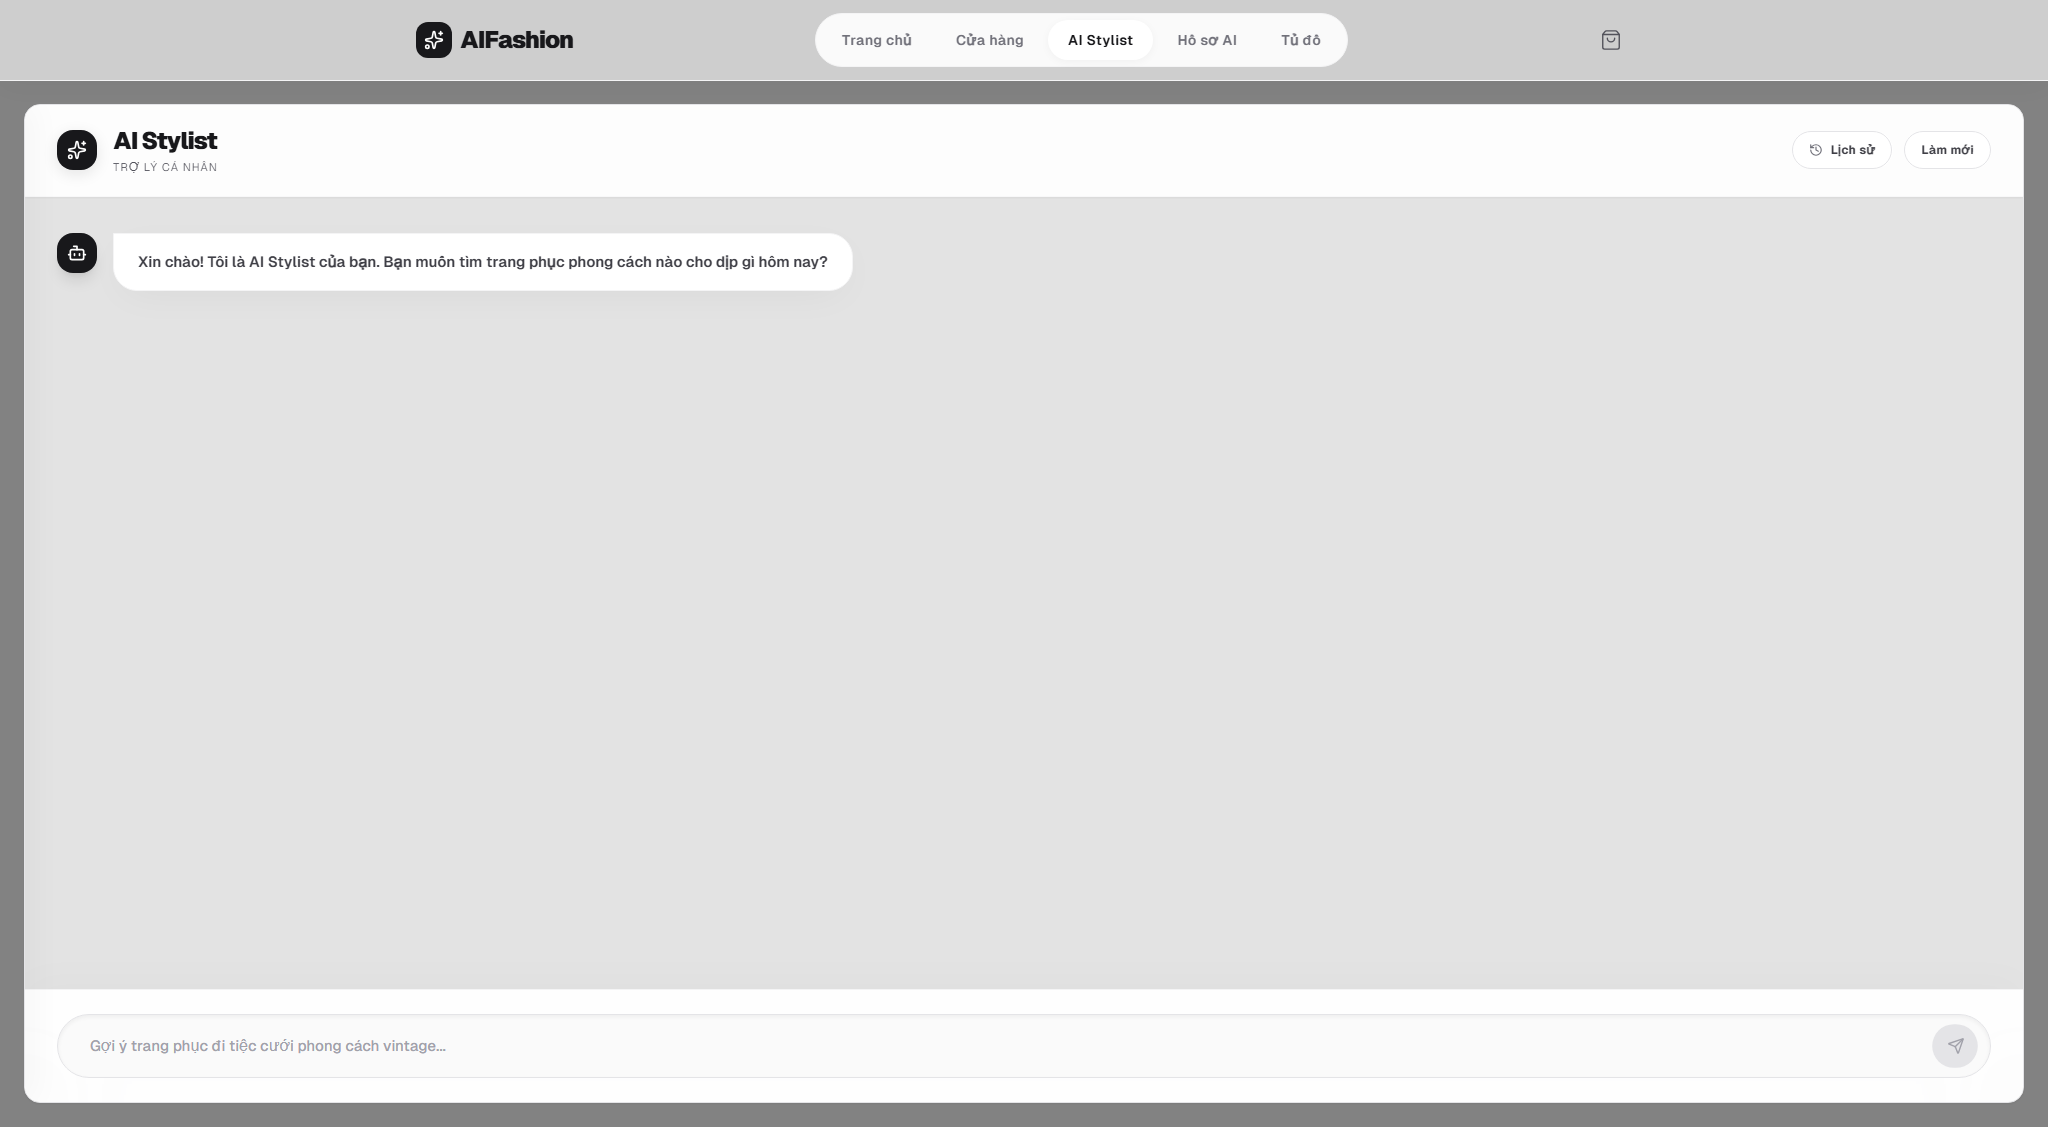
\includegraphics[width=0.95\textwidth]{Images/screenshots/ui_ai_stylist.png}
    \caption{Giao diện AI Stylist và khu vực hội thoại}
    \label{fig:ui-ai-stylist}
\end{figure}

\begin{figure}[H]
    \centering
    \begin{minipage}[t]{0.49\textwidth}
        \centering
        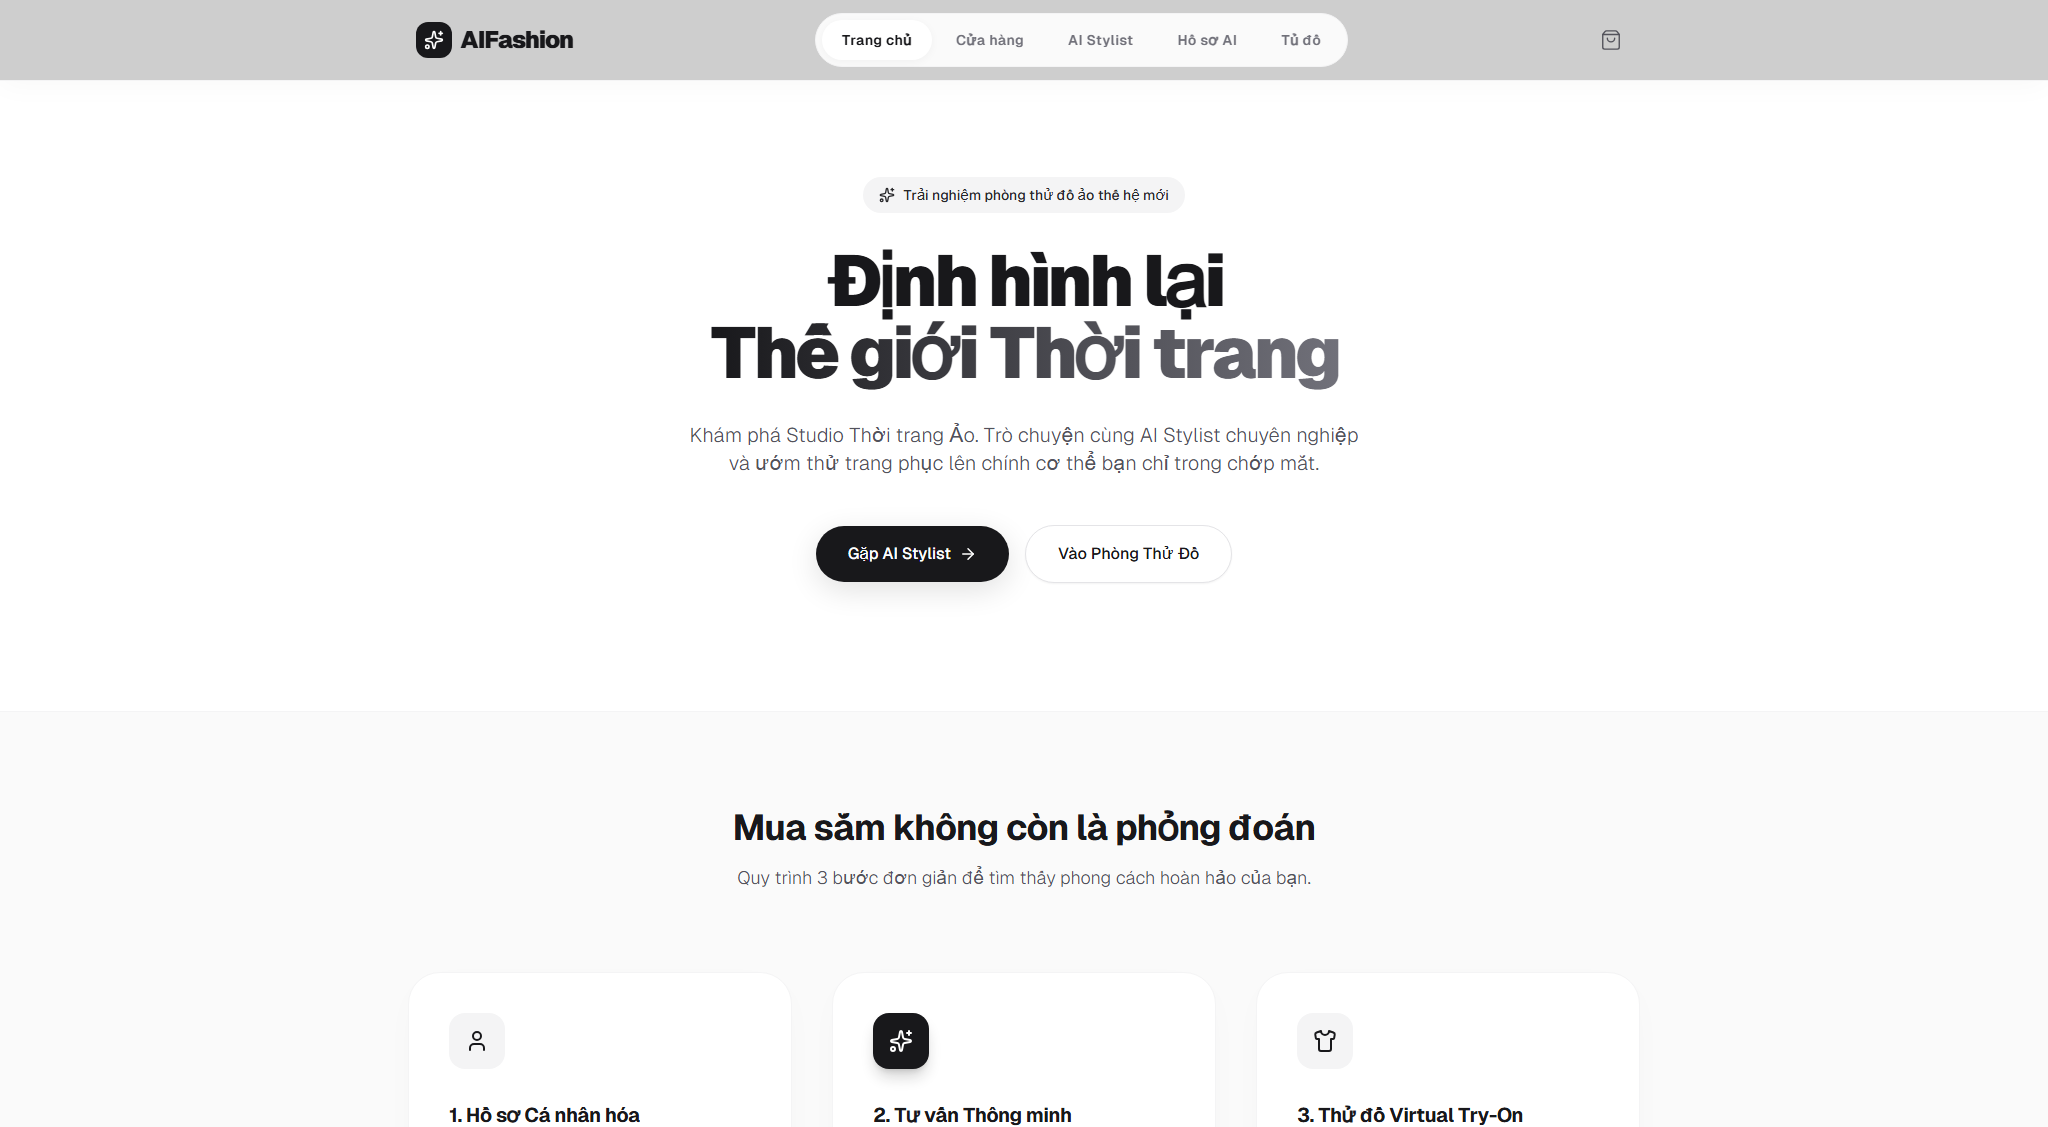
\includegraphics[width=\linewidth]{Images/screenshots/ui_home.png}
        \par\smallskip
        \small (a) Trang chủ
    \end{minipage}
    \hfill
    \begin{minipage}[t]{0.49\textwidth}
        \centering
        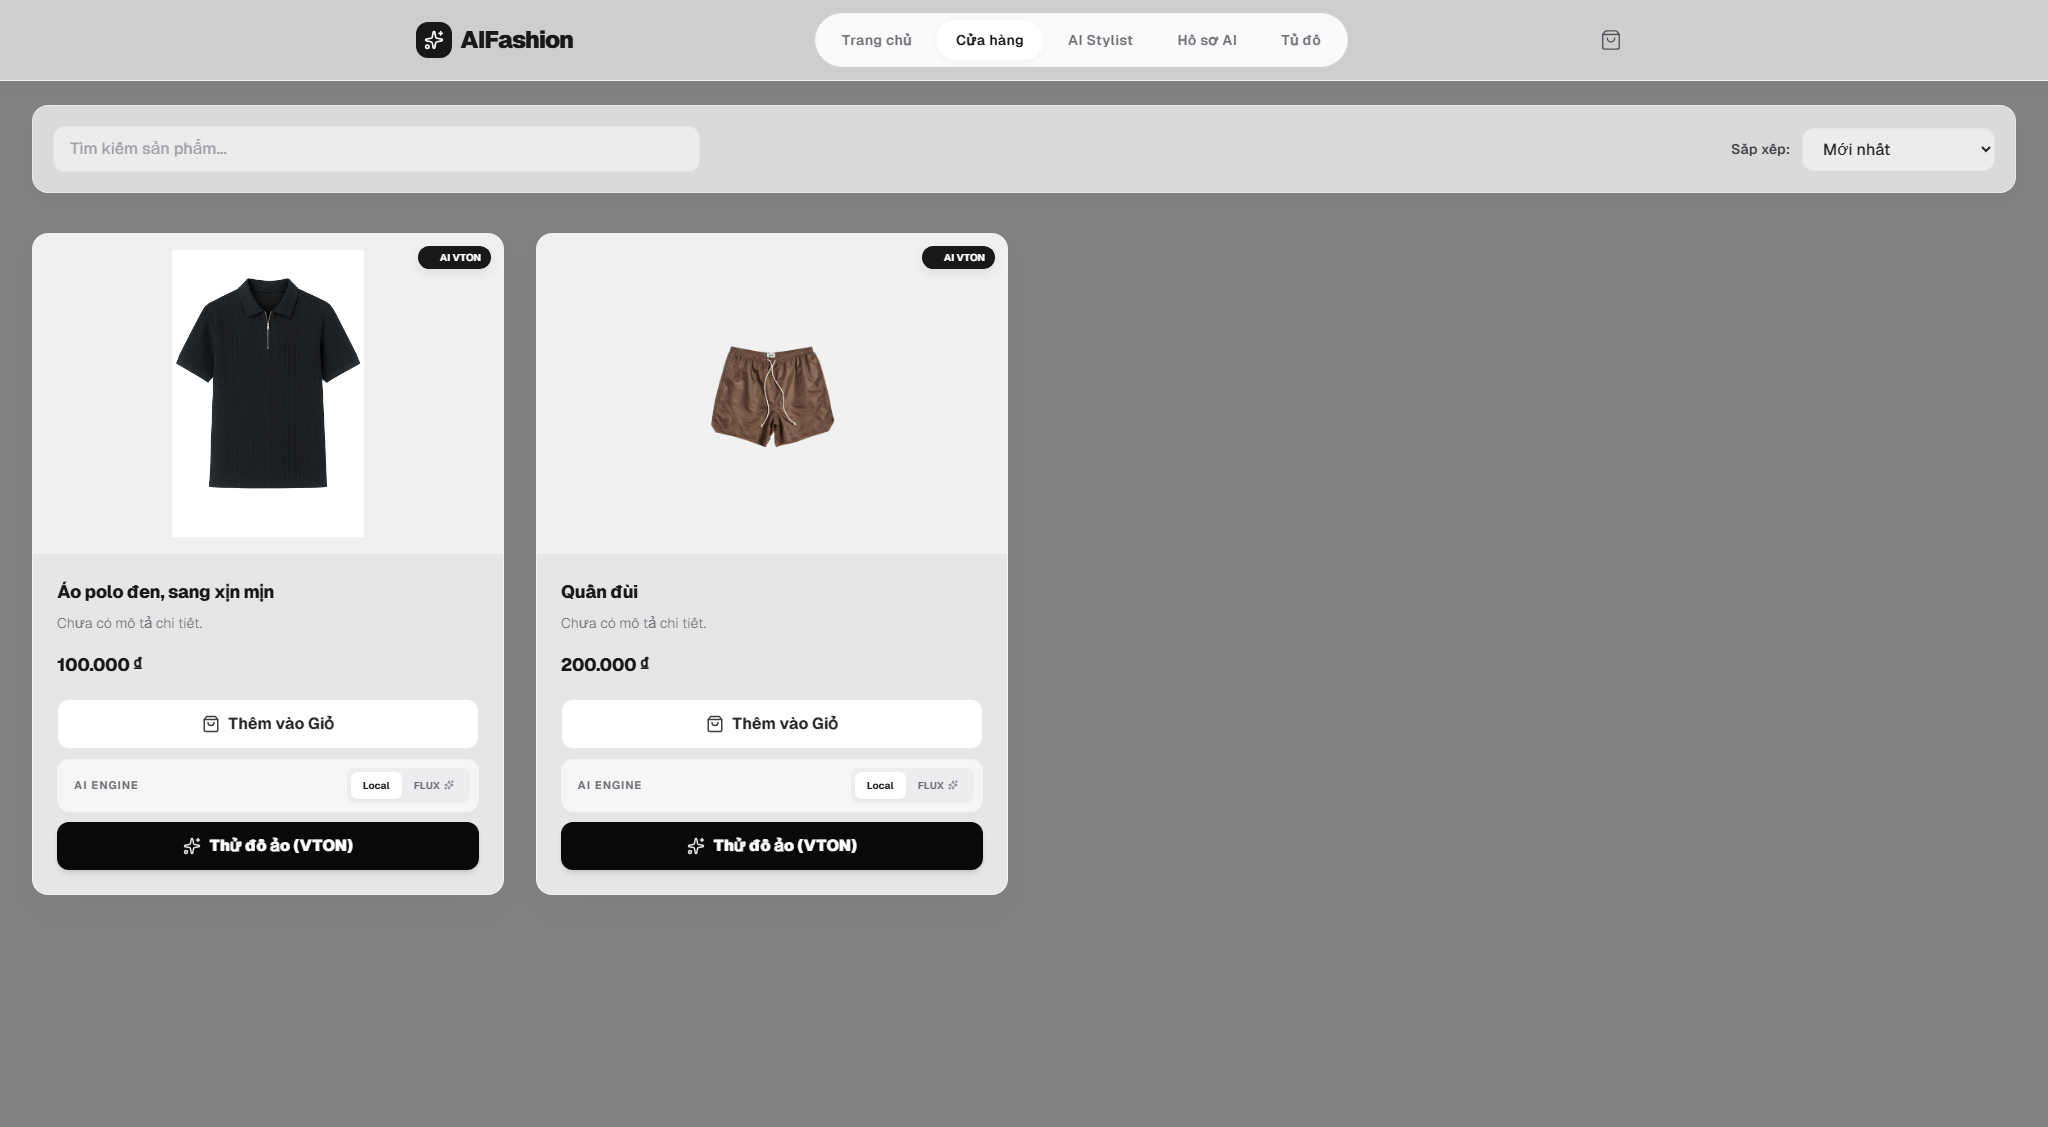
\includegraphics[width=\linewidth]{Images/screenshots/ui_products.png}
        \par\smallskip
        \small (b) Trang cửa hàng
    \end{minipage}
    \caption{Các màn hình cửa hàng chính}
    \label{fig:ui-storefront}
\end{figure}

\begin{figure}[H]
    \centering
    \begin{minipage}[t]{0.49\textwidth}
        \centering
        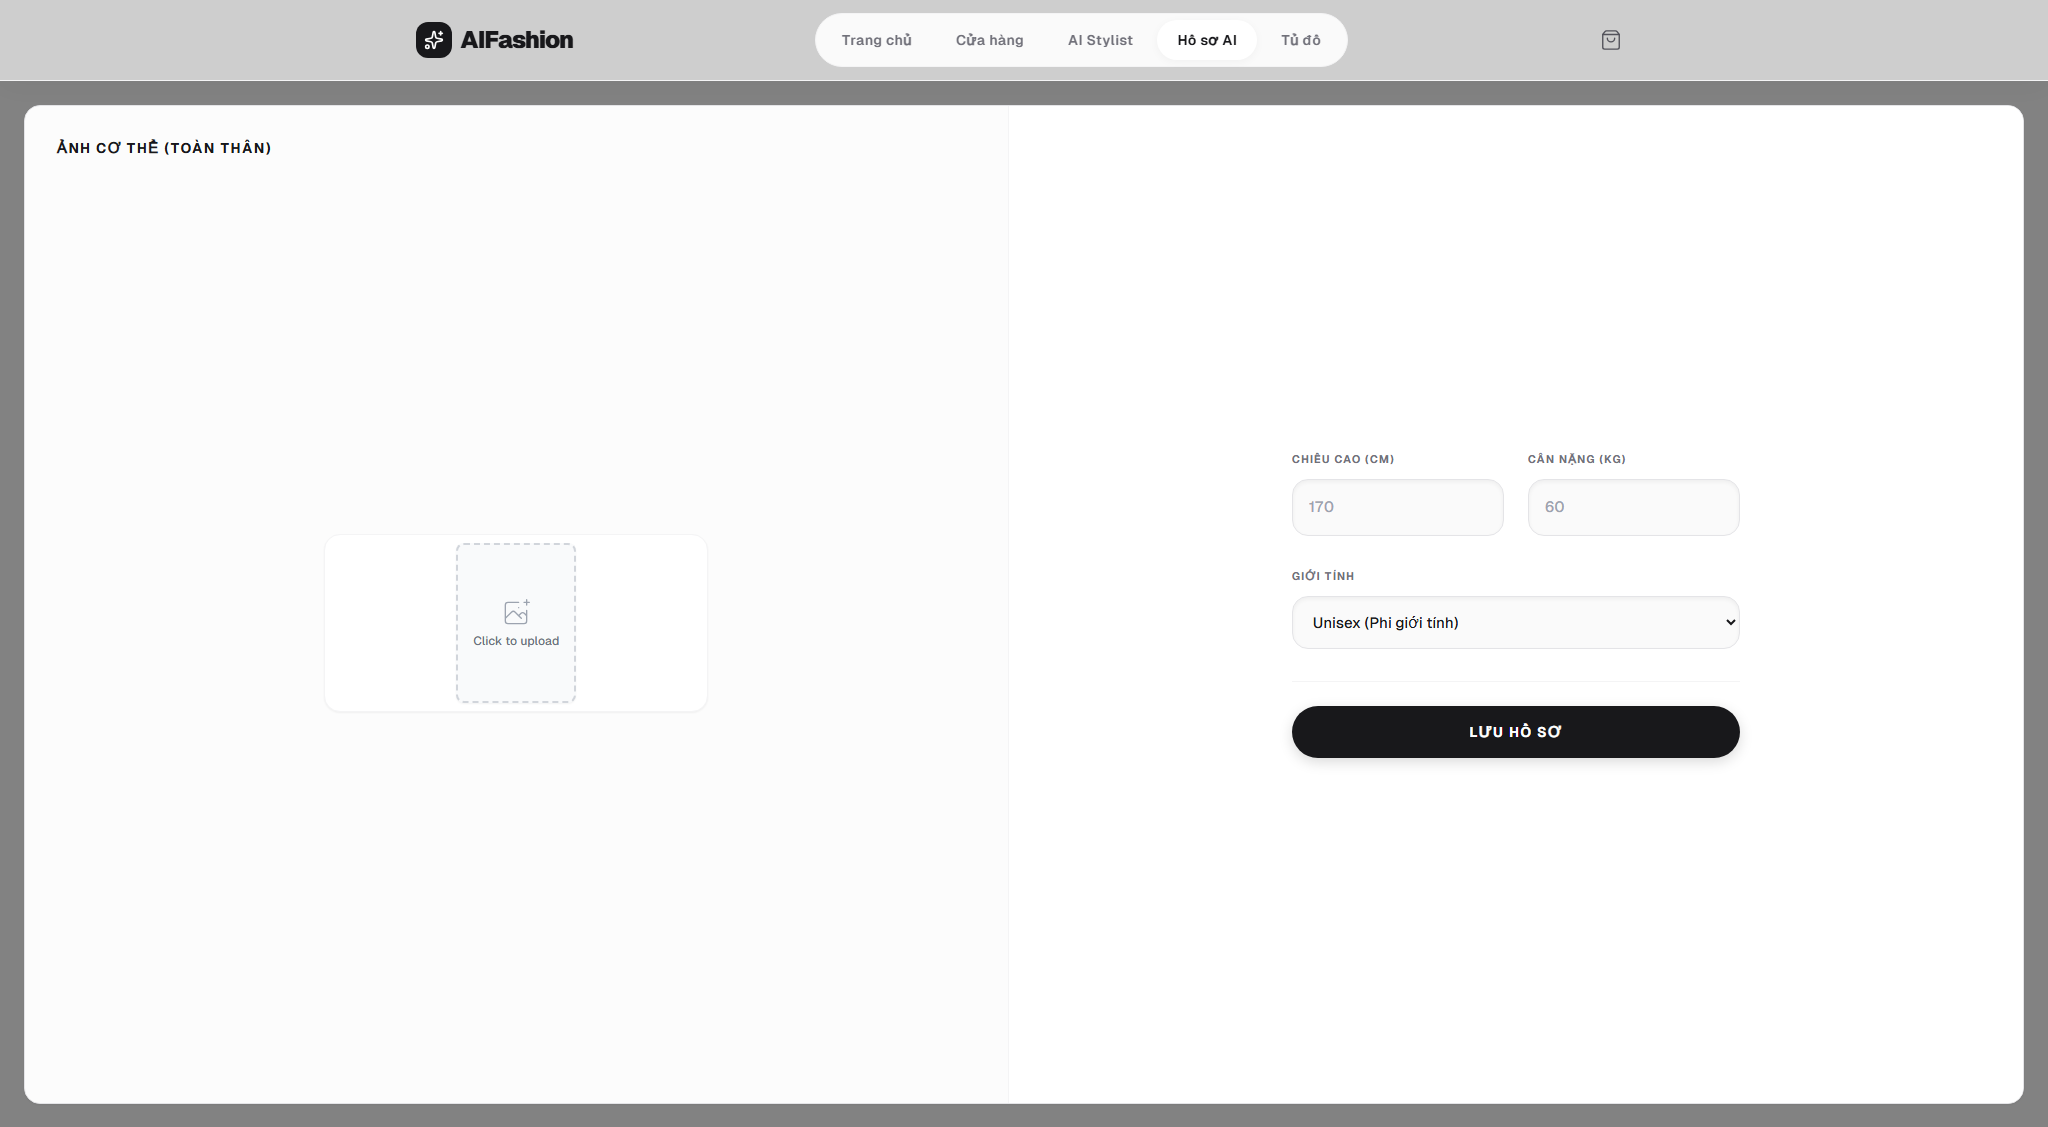
\includegraphics[width=\linewidth]{Images/screenshots/ui_ai_profile.png}
        \par\smallskip
        \small (a) Hồ sơ AI
    \end{minipage}
    \hfill
    \begin{minipage}[t]{0.49\textwidth}
        \centering
        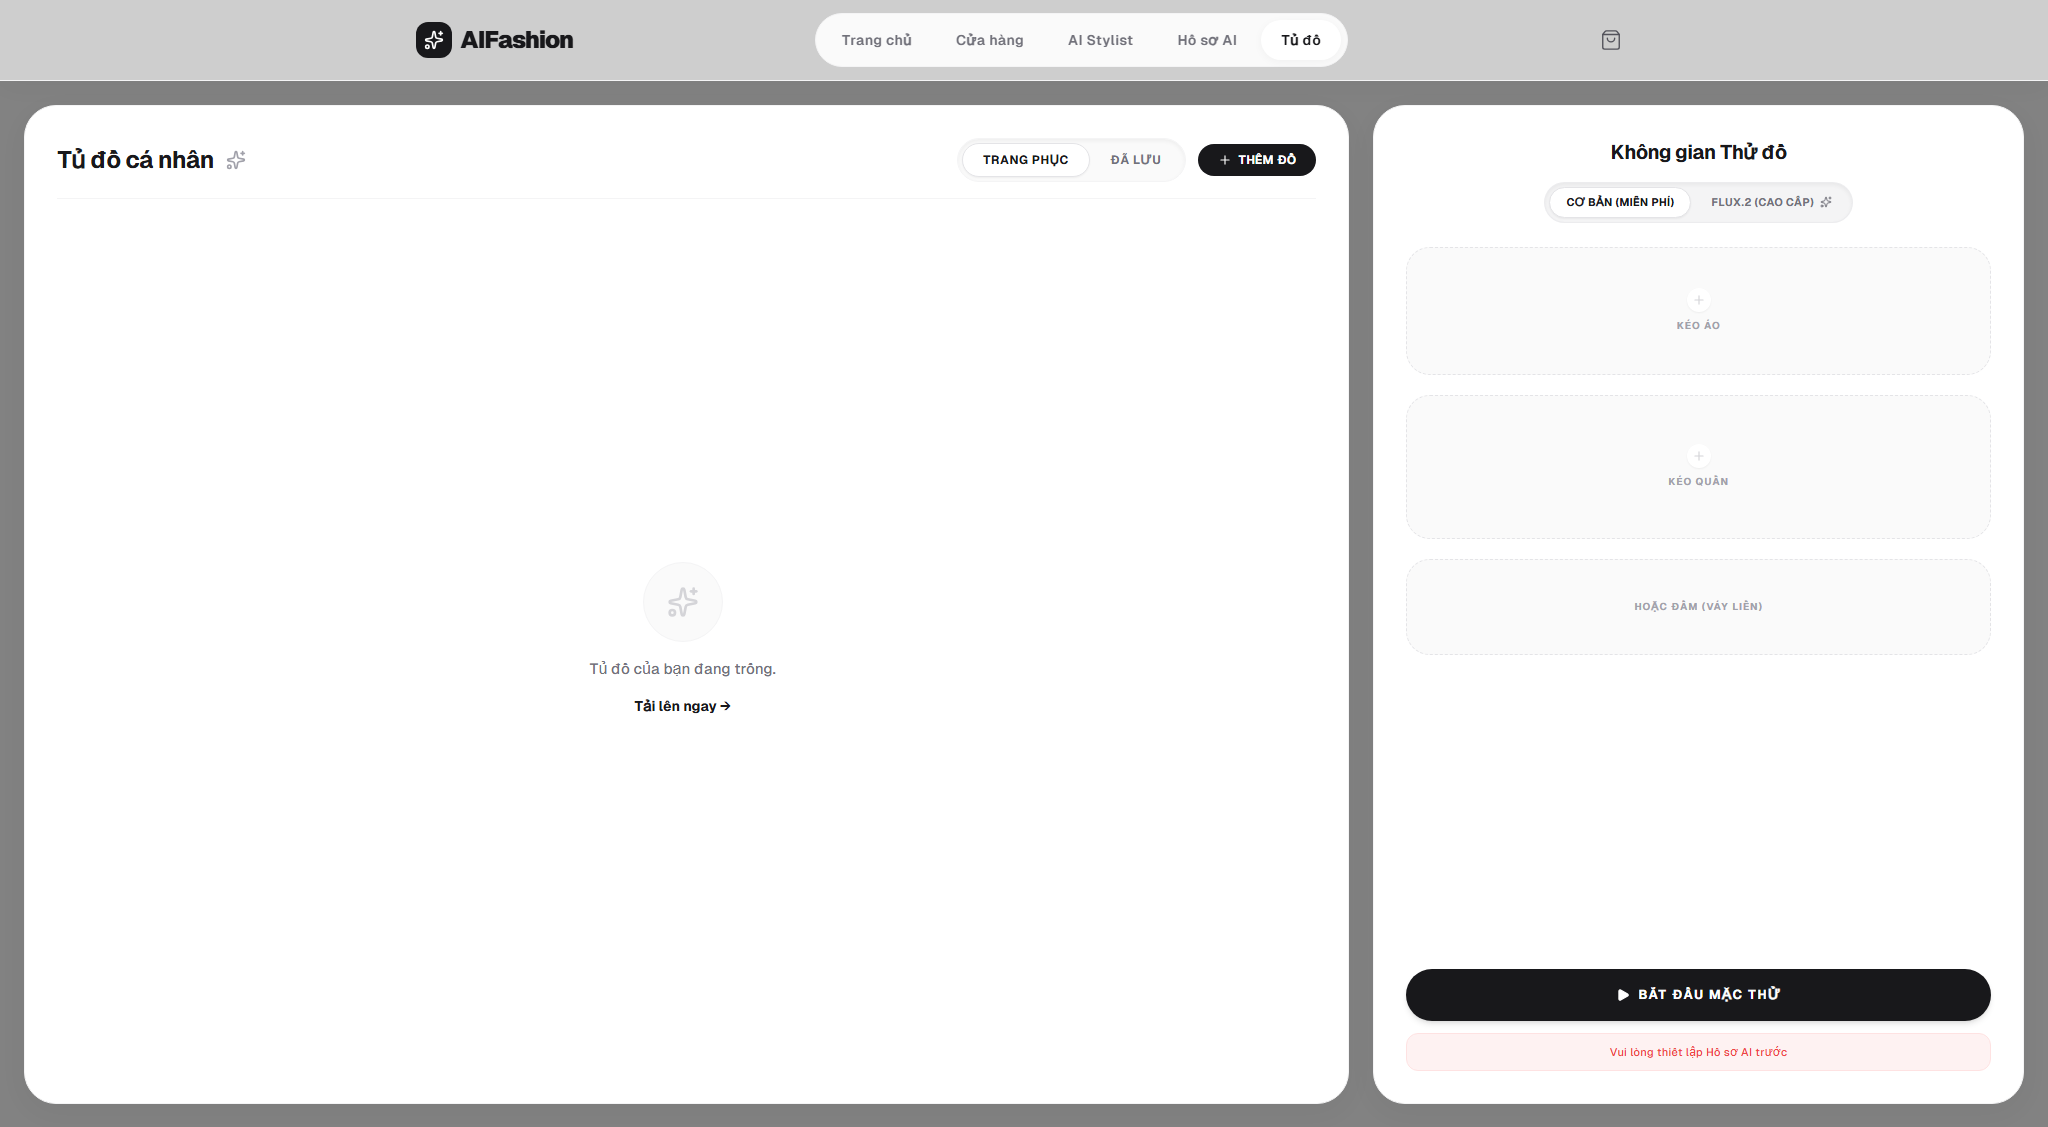
\includegraphics[width=\linewidth]{Images/screenshots/ui_wardrobe.png}
        \par\smallskip
        \small (b) Tủ đồ và không gian thử đồ
    \end{minipage}
    \caption{Giao diện hồ sơ AI và tủ đồ cá nhân}
    \label{fig:ui-profile-wardrobe}
\end{figure}

\medskip

Giao diện chỉ đảm nhiệm trình bày và thu thập thao tác. Các quyết định nghiệp vụ như kiểm tra sản phẩm, tạo tác vụ VTON hoặc lưu phiên tư vấn được đặt tại MedusaJS.

\section{Cài đặt hệ thống nghiệp vụ MedusaJS}

MedusaJS 2.14 và TypeScript được sử dụng để quản lý dữ liệu thương mại điện tử, cung cấp API cho giao diện và điều phối các luồng AI \cite{medusa}. Mô-đun \code{aiPersonalization} tập trung các thực thể hồ sơ AI, tủ đồ, phiên tư vấn và tác vụ VTON trong một phạm vi nghiệp vụ riêng.

\medskip

Các tuyến API tùy chỉnh dưới \code{apps/api-medusa/src/api/v1} được chia theo chức năng. Nhóm hồ sơ và tủ đồ tiếp nhận ảnh, chuẩn hóa định dạng, lưu bản ghi và phát sự kiện đồng bộ vector. Nhóm AI Stylist gọi dịch vụ AI, kiểm tra sản phẩm được đề xuất, bổ sung dữ liệu giao dịch và lưu phiên tư vấn. Nhóm VTON tạo tác vụ, phát thông điệp RabbitMQ và cập nhật trạng thái khi nhận kết quả.

\medskip

Cách tổ chức này đặt quyền kiểm soát nghiệp vụ tại Medusa. Dịch vụ AI chỉ trả kết quả phân tích hoặc sinh ảnh; dữ liệu sản phẩm, phiên người dùng và trạng thái tác vụ vẫn được Medusa kiểm tra trước khi cung cấp cho giao diện.

\section{Cài đặt dịch vụ AI FastAPI}

Dịch vụ AI được xây dựng bằng FastAPI và đặt trong \code{apps/ai-service} \cite{fastapi}. Khi khởi động, dịch vụ kết nối LanceDB, đăng ký các tuyến API nội bộ và khởi tạo bộ tiêu thụ RabbitMQ. Những phụ thuộc VTON có kích thước lớn được nạp trong luồng nền để các thành phần cơ bản có thể sẵn sàng trước.

\medskip

Ba nhóm thông điệp chính được xử lý độc lập: đồng bộ sản phẩm, đồng bộ tủ đồ và tác vụ VTON. Các lược đồ Pydantic kiểm soát dữ liệu đầu vào và đầu ra của API nội bộ, giúp phát hiện sớm trường thiếu hoặc sai kiểu trước khi dữ liệu được chuyển giữa Medusa, mô hình AI và LanceDB.

\section{Tích hợp các luồng chức năng chính}

Sau khi ba thành phần chính được cài đặt, hệ thống tích hợp chúng thành các luồng chức năng xuyên suốt giữa giao diện, Medusa, RabbitMQ, LanceDB và dịch vụ AI.

\medskip

\subsection{Đồng bộ dữ liệu sang LanceDB}

Khi sản phẩm được tạo hoặc cập nhật, \code{product-sync.ts} phát thông điệp vào \code{product_metadata_sync} qua RabbitMQ \cite{rabbitmq}. Dịch vụ AI sử dụng Gemini để trích xuất thuộc tính thời trang, tạo vector nhúng bằng CLIP và ghi dữ liệu vào \code{products_vector}. Bản ghi cũ của cùng \code{product_id} được thay thế trước khi ghi mới để tránh trùng lặp.

\medskip

Tủ đồ cá nhân được đồng bộ theo quy trình tương tự. Ảnh do người dùng tải lên được phân tích để suy luận danh mục, màu sắc, họa tiết và chất liệu; kết quả cùng vector nhúng được lưu trong \code{closet_vector}. Mỗi bản ghi luôn gắn với định danh chủ sở hữu để giới hạn phạm vi truy hồi.

\subsection{AI Stylist}

AI Stylist sử dụng \code{GeminiAnalyzerAdapter} để phân tích truy vấn, sinh phương án phối đồ và trích xuất thuộc tính thời trang. Sau bước phân tích ý định, \code{VectorSearch.global_search} truy hồi ứng viên từ sản phẩm cửa hàng và tủ đồ cá nhân. Tập ứng viên được truyền cho Gemini để sinh phương án phối đồ có cấu trúc.

\medskip

Chỉ dẫn cho mô hình được tách thành hai nhiệm vụ: phân tích yêu cầu và lựa chọn trang phục. Mô hình chỉ được chọn sản phẩm thuộc tập ứng viên, ưu tiên tủ đồ cá nhân và giới hạn số lớp có thể thử bằng VTON. Medusa tiếp tục kiểm tra định danh và bổ sung dữ liệu giao dịch, nhờ đó phần giải thích luôn gắn với sản phẩm thực tế.

\subsection{Virtual Try-On và cập nhật kết quả bằng SSE}

VTON hỗ trợ hai bộ xử lý. \code{LocalCatVTONAdapter} tải CatVTON, tạo mặt nạ khi cần và chạy suy luận trên máy cục bộ \cite{catvton}. \code{CloudFluxVTONAdapter} chuyển ảnh thành dữ liệu phù hợp, gọi FLUX.2 qua Replicate và tải ảnh kết quả về dịch vụ AI \cite{replicate}. Cả hai bộ xử lý tuân theo cùng hợp đồng giao tiếp nên phần điều phối không phụ thuộc trực tiếp vào mô hình cụ thể.

\medskip

Ảnh kết quả được lưu trong thư mục dữ liệu của dịch vụ AI và cung cấp qua địa chỉ tệp tĩnh, chẳng hạn \code{/static/vton/result_<job_id>.png}. Đây là giải pháp phù hợp với phạm vi bản triển khai tối thiểu; môi trường vận hành thực tế cần chuyển sang kho đối tượng dùng chung.

\medskip

Giao diện mở \code{EventSource} tới \code{/v1/stream/vision-results} trước khi tạo tác vụ. Khi Medusa nhận thông điệp từ \code{ai_vision_results}, \code{VisionOrchestrator} cập nhật trạng thái và \code{VisionSSEManager} gửi sự kiện \code{vision_update} tới người dùng tương ứng \cite{sse-mdn}. Thứ tự này giảm khả năng bỏ lỡ sự kiện và cho phép giao diện phản ánh liên tục trạng thái chờ, đang xử lý, hoàn tất hoặc thất bại.

\subsection{Thanh toán mô phỏng bằng Saga}

Luồng thanh toán phía Medusa được cài đặt bằng Medusa Workflow SDK. Quy trình gồm giữ tồn kho, tạo đơn hàng chờ xử lý, xử lý thanh toán mô phỏng và hoàn tất đơn hàng. Khi bước thanh toán thất bại, các hàm bù được thực thi để kiểm tra khả năng hoàn tác của quy trình Saga.

\medskip

Phần cài đặt này mới hoàn thành ở phía hệ thống nghiệp vụ; tuyến gọi từ giao diện chưa được thống nhất hoàn toàn với API Medusa. Vì vậy, thanh toán hiện đóng vai trò minh họa quy trình nghiệp vụ và chưa được xem là quy trình đầu cuối hoàn chỉnh.

\clearpage

\chapter{Kết quả thực nghiệm và đánh giá}

Chương này trình bày kết quả triển khai các chức năng chính, thực nghiệm Virtual Try-On và đánh giá những quyết định kiến trúc của hệ thống. Phần thực nghiệm tập trung vào khả năng tạo ảnh thử đồ và thời gian xử lý của CatVTON cục bộ so với FLUX.2 qua Replicate trên cùng bộ ảnh đầu vào.

\medskip

\section{Kết quả triển khai chức năng}

Các luồng chức năng được kiểm tra từ giao diện người dùng tới hệ thống nghiệp vụ và dịch vụ AI. Kết quả tổng hợp trong Bảng~\ref{tab:functional-results} cho thấy hệ thống đã hiện thực được chuỗi tương tác chính của một nền tảng thương mại điện tử thời trang tích hợp AI.

\medskip

\begin{table}[H]
\centering
\small
\caption{Kết quả kiểm tra các chức năng chính}
\label{tab:functional-results}
\begin{tabularx}{\textwidth}{L{3.2cm}L{3.0cm}Y}
\toprule
\textbf{Chức năng} & \textbf{Kết quả} & \textbf{Minh chứng triển khai} \\
\midrule
Cửa hàng và giỏ hàng & Đạt phạm vi tối thiểu & Hiển thị sản phẩm từ Medusa Store API, tìm kiếm, sắp xếp, thêm sản phẩm và thay đổi số lượng. \\
\addlinespace
Hồ sơ AI và tủ đồ & Đạt phạm vi tối thiểu & Lưu ảnh cơ thể và thông tin hồ sơ; thêm, hiển thị và xóa trang phục cá nhân. \\
\addlinespace
AI Stylist & Hoàn thành luồng chính & Phân tích yêu cầu, truy hồi dữ liệu từ LanceDB, sinh phương án phối đồ có cấu trúc và bổ sung dữ liệu sản phẩm thực. \\
\addlinespace
Thay thế trang phục & Đạt phạm vi tối thiểu & Tìm kiếm trang phục tương đồng và loại trừ các mục đã có trong phương án phối đồ. \\
\addlinespace
VTON cục bộ & Hoạt động & CatVTON xử lý tác vụ từ RabbitMQ, lưu ảnh kết quả và trả trạng thái về Medusa. \\
\addlinespace
VTON đám mây & Hoạt động & FLUX.2 tiếp nhận nhiều ảnh tham chiếu trong một yêu cầu và trả ảnh kết quả qua Replicate. \\
\addlinespace
Cập nhật kết quả VTON & Hoạt động & Medusa nhận \code{ai_vision_results} và phát sự kiện \code{vision_update} tới giao diện bằng SSE. \\
\addlinespace
Thanh toán mô phỏng & Đã triển khai phía Medusa, chưa hoàn tất tích hợp đầu cuối & Quy trình mô phỏng các bước nghiệp vụ và hỗ trợ kiểm tra hoàn tác khi thanh toán thất bại. \\
\bottomrule
\end{tabularx}
\end{table}

\medskip

Các ảnh giao diện tại Hình~\ref{fig:ui-ai-stylist}, Hình~\ref{fig:ui-storefront} và Hình~\ref{fig:ui-profile-wardrobe} cho thấy các chức năng AI được tích hợp trực tiếp vào hành trình mua sắm thay vì tồn tại như các chức năng minh họa tách rời. AI Stylist trả về dữ liệu có thể thao tác; hồ sơ AI và tủ đồ cung cấp đầu vào cho VTON; kết quả thử đồ được gửi về giao diện sau khi tác vụ bất đồng bộ hoàn tất.

\section{Điều kiện thực nghiệm Virtual Try-On}

Thực nghiệm sử dụng một ảnh người dùng, một ảnh trang phục phần trên và một ảnh trang phục phần dưới. CatVTON thực hiện hai bước tuần tự: thay trang phục phần trên, sau đó sử dụng ảnh trung gian làm đầu vào cho bước thay trang phục phần dưới. FLUX.2 nhận đồng thời ảnh người dùng và hai ảnh trang phục tham chiếu để tạo kết quả toàn bộ trang phục trong một yêu cầu.

\medskip

\begin{figure}[H]
    \centering
    \begin{minipage}[t]{0.32\textwidth}
        \centering
        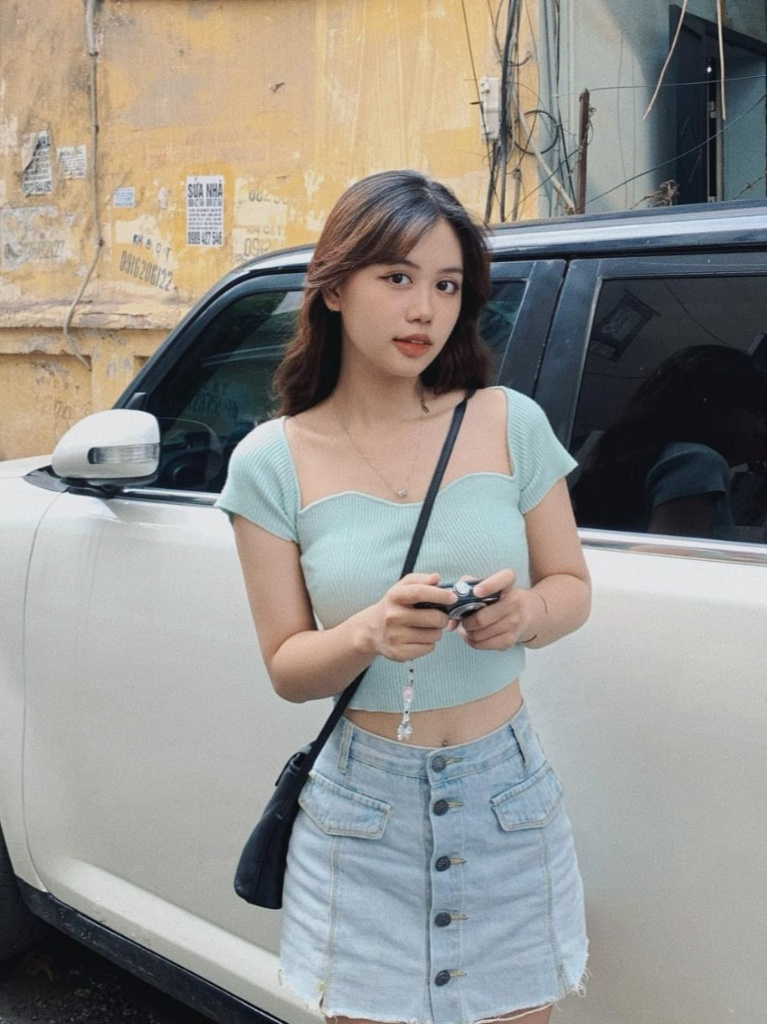
\includegraphics[height=5.6cm,keepaspectratio]{Images/vton/human_input.jpg}
        \par\smallskip
        \small (a) Ảnh người dùng
    \end{minipage}
    \begin{minipage}[t]{0.32\textwidth}
        \centering
        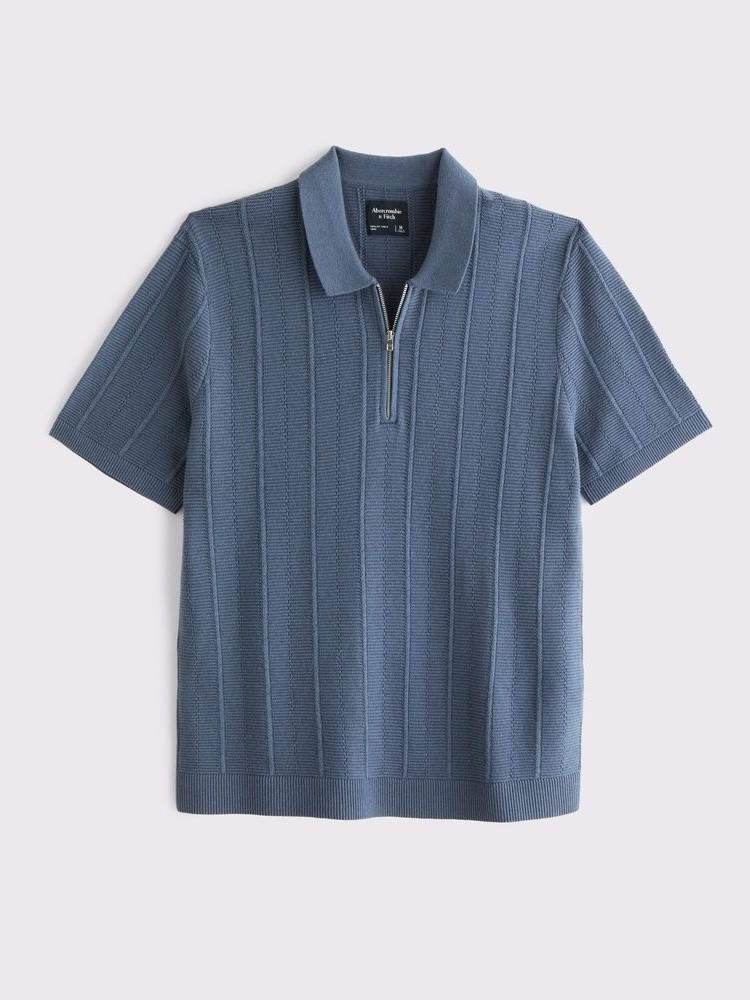
\includegraphics[height=5.6cm,keepaspectratio]{Images/vton/garment_upper.png}
        \par\smallskip
        \small (b) Trang phục phần trên
    \end{minipage}
    \begin{minipage}[t]{0.32\textwidth}
        \centering
        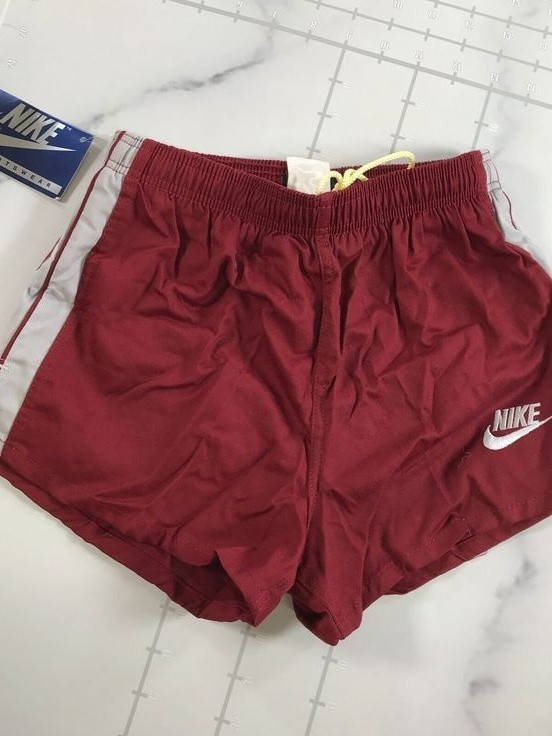
\includegraphics[height=5.6cm,keepaspectratio]{Images/vton/garment_lower.png}
        \par\smallskip
        \small (c) Trang phục phần dưới
    \end{minipage}
    \caption{Ảnh đầu vào cho thực nghiệm thử đồ ảo}
    \label{fig:vton-inputs}
\end{figure}

\medskip

CatVTON cục bộ được thực thi trên máy có GPU NVIDIA GeForce RTX 5060 với 8 GB VRAM, 16 GB RAM và CPU AMD Ryzen 9 8940HX. Mỗi bước sử dụng 25 vòng suy luận, \code{scale=2.5}, AutoMask và hậu xử lý repaint. Thời gian FLUX.2 được đo từ khi gửi yêu cầu tới Replicate đến khi nhận được ảnh kết quả.

\section{Kết quả thực nghiệm}

Hình~\ref{fig:vton-results} trình bày kết quả của hai phương án xử lý. CatVTON giữ ổn định khuôn mặt, tư thế, bàn tay và phần lớn bối cảnh gốc qua hai bước tuần tự. FLUX.2 tạo lại toàn bộ trang phục trong một lần xử lý, đồng thời thay đổi một số chi tiết về chất liệu áo, phụ kiện và đặc điểm hình ảnh.

\medskip

\begin{figure}[H]
    \centering
    \begin{minipage}[t]{0.32\textwidth}
        \centering
        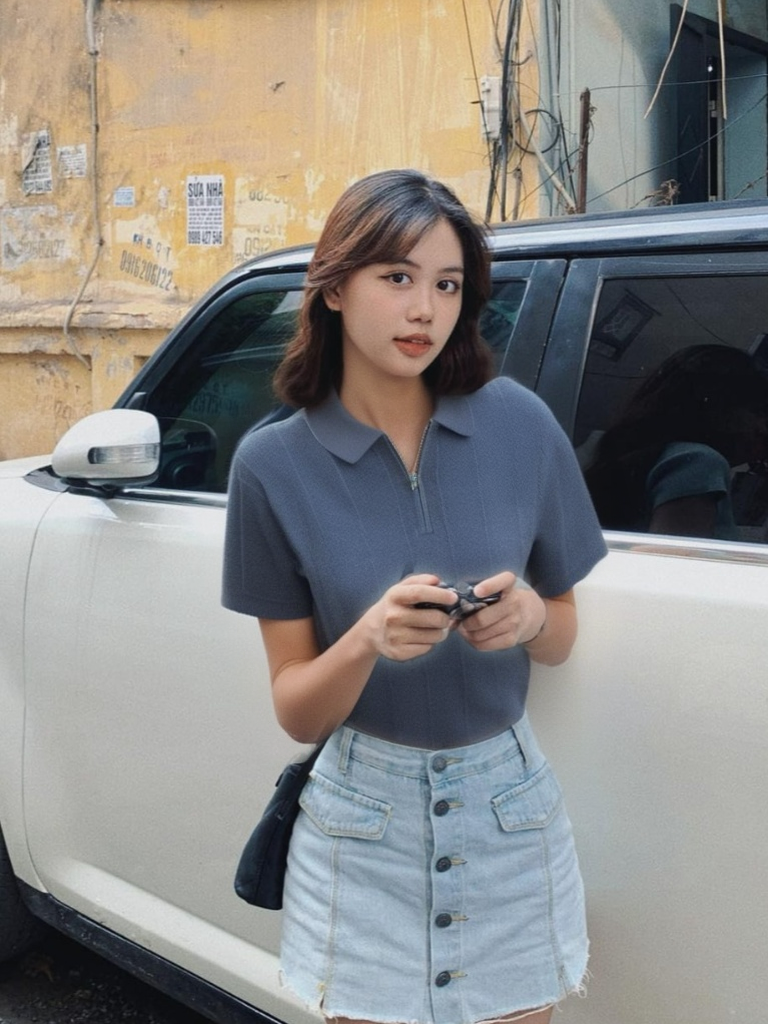
\includegraphics[height=6.4cm,keepaspectratio]{Images/vton/catvton_upper_result.png}
        \par\smallskip
        \small (a) CatVTON sau bước \code{upper}
    \end{minipage}
    \begin{minipage}[t]{0.32\textwidth}
        \centering
        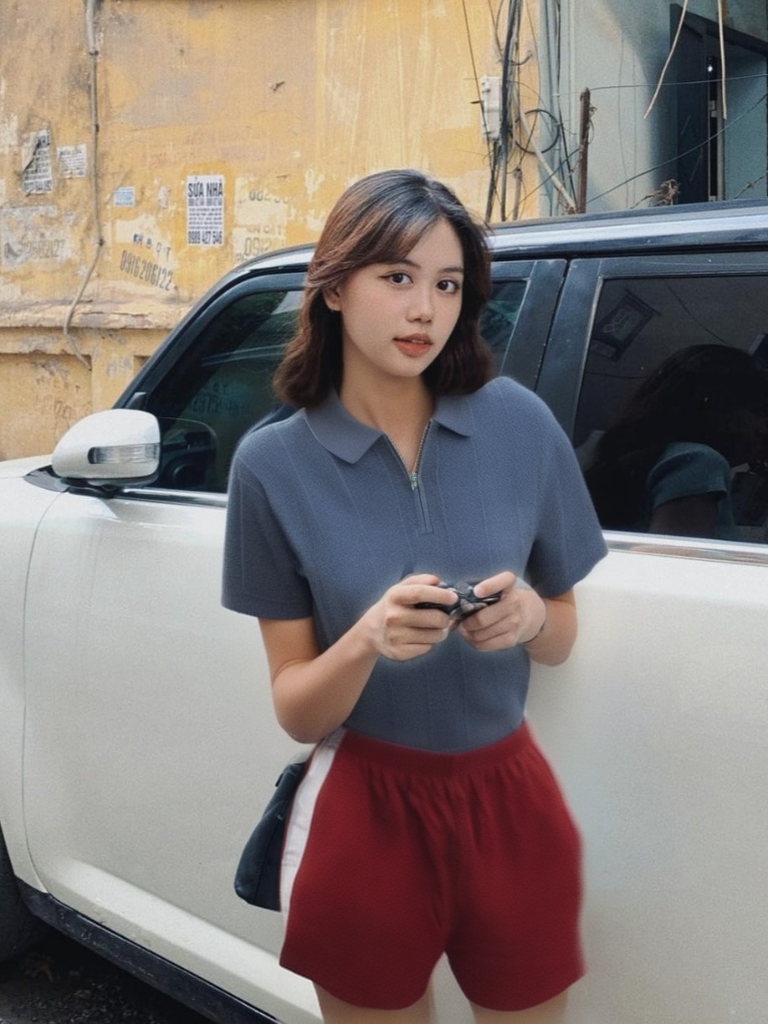
\includegraphics[height=6.4cm,keepaspectratio]{Images/vton/catvton_outfit_result.png}
        \par\smallskip
        \small (b) CatVTON sau bước \code{lower}
    \end{minipage}
    \begin{minipage}[t]{0.32\textwidth}
        \centering
        
\includegraphics[height=6.4cm,keepaspectratio]{Images/vton/flux2_outfit_result.png}
        \par\smallskip
        \small (c) Kết quả FLUX.2
    \end{minipage}
    \caption{Kết quả thử đồ của CatVTON cục bộ và FLUX.2 đám mây}
    \label{fig:vton-results}
\end{figure}

\medskip

Log xử lý cho thấy CatVTON hoàn thành bước thay trang phục phần trên trong khoảng 33 giây và bước thay trang phục phần dưới trong khoảng 31 giây. Tổng thời gian suy luận của chuỗi hai bước là khoảng 64 giây. Với cùng bộ ảnh tham chiếu, FLUX.2 trả kết quả toàn bộ trang phục sau khoảng 21 giây.

\medskip

\begin{table}[H]
\centering
\small
\caption{Thời gian xử lý Virtual Try-On trong thực nghiệm}
\label{tab:vton-observed-time}
\begin{tabularx}{\textwidth}{L{3.4cm}L{2.3cm}L{2.8cm}Y}
\toprule
\textbf{Phương án xử lý} & \textbf{Số bước} & \textbf{Thời gian} & \textbf{Đặc điểm} \\
\midrule
CatVTON phần trên & 25 vòng suy luận & Khoảng 33 giây & Tạo ảnh trung gian, giữ nguyên trang phục phần dưới. \\
\addlinespace
CatVTON phần dưới & 25 vòng suy luận & Khoảng 31 giây & Sử dụng ảnh kết quả của bước phần trên làm đầu vào. \\
\addlinespace
CatVTON toàn bộ trang phục & Hai bước tuần tự & Khoảng 64 giây & Tổng thời gian suy luận của hai bước. \\
\addlinespace
FLUX.2 toàn bộ trang phục & Một yêu cầu & Khoảng 21 giây & Xử lý đồng thời nhiều ảnh tham chiếu qua Replicate. \\
\bottomrule
\end{tabularx}
\end{table}

\section{Phân tích kết quả thực nghiệm}

Xét về thời gian xử lý, FLUX.2 hoàn thành toàn bộ trang phục nhanh hơn CatVTON hai bước khoảng 43 giây, tương ứng giảm gần 67\% thời gian so với chuỗi CatVTON. Chênh lệch này xuất phát chủ yếu từ cách tổ chức tác vụ: CatVTON phải thực hiện hai lần suy luận nối tiếp, trong khi FLUX.2 tiếp nhận nhiều ảnh tham chiếu trong một yêu cầu.

\medskip

Xét về mức độ bảo toàn ảnh gốc, CatVTON giữ khuôn mặt, tư thế, bàn tay, túi đeo và bối cảnh ổn định hơn. Bước thay phần dưới tiếp tục sử dụng kết quả của bước trước nên phần áo đã tạo được duy trì. Tuy nhiên, xử lý tuần tự làm tổng độ trễ tăng theo số vùng trang phục và có khả năng tích lũy sai lệch qua từng bước.

\medskip

FLUX.2 tạo kết quả có độ hoàn thiện thị giác cao và tái hiện rõ đặc điểm của quần tham chiếu, nhưng mô hình cũng thay đổi kết cấu áo, tỷ lệ cơ thể và một số chi tiết phụ kiện. Điều này phù hợp với bản chất của một mô hình sinh và chỉnh sửa ảnh tổng quát: kết quả có tính linh hoạt cao nhưng mức độ bảo toàn chính xác từng vùng ảnh khó kiểm soát hơn mô hình VTON chuyên biệt.

\medskip

Kết quả cho thấy hai phương án phù hợp với các mục tiêu khác nhau. CatVTON thích hợp khi cần chủ động dữ liệu, kiểm soát quá trình suy luận và giữ ổn định ảnh gốc. FLUX.2 phù hợp khi ưu tiên thời gian phản hồi và xử lý toàn bộ trang phục trong một yêu cầu. Việc hỗ trợ cả hai phương án giúp hệ thống lựa chọn theo điều kiện hạ tầng và yêu cầu trải nghiệm.

\section{Đánh giá kiến trúc}

Việc tách Medusa khỏi dịch vụ AI giúp các tác vụ sinh ảnh không chặn luồng thương mại điện tử. RabbitMQ tiếp nhận tác vụ VTON và giới hạn số thông điệp chưa xác nhận tại mỗi bộ tiêu thụ, nhờ đó tải xử lý phù hợp hơn với tài nguyên GPU. SSE hoàn thiện luồng bất đồng bộ bằng cách gửi trạng thái và ảnh kết quả về đúng giao diện đang chờ.

\medskip

Luồng AI Stylist sử dụng truy hồi trước khi sinh phương án phối đồ. Cách tổ chức này giới hạn tập sản phẩm mà mô hình được lựa chọn và cho phép Medusa kiểm tra lại dữ liệu giao dịch trước khi trả về giao diện. Mẫu thiết kế adapter tiếp tục giảm phụ thuộc trực tiếp vào Gemini, CatVTON hoặc Replicate, tạo điều kiện thay đổi mô hình mà không làm thay đổi toàn bộ luồng nghiệp vụ.

\medskip

Kiến trúc hiện tại đáp ứng mục tiêu của một bản triển khai kỹ thuật tối thiểu có nhiều thành phần tích hợp. Các ranh giới dịch vụ, hợp đồng dữ liệu và cơ chế xử lý bất đồng bộ đã được thể hiện trong mã nguồn và kết quả thực nghiệm. Tuy nhiên, để vận hành ở quy mô lớn hơn, hệ thống cần hoàn thiện bảo mật, độ tin cậy thông điệp và lưu trữ dùng chung.

\section{Hạn chế}

Cơ chế xác thực người dùng chưa hoàn chỉnh; một số API và giao diện vẫn sử dụng định danh mặc định. Luồng thanh toán mới mô phỏng quy trình Saga và đường dẫn gọi từ giao diện chưa thống nhất với API Medusa. Ảnh tải lên và ảnh kết quả VTON được lưu trên máy chạy dịch vụ, chưa sử dụng kho đối tượng dùng chung.

\medskip

Trong luồng VTON cục bộ nhiều bước, địa chỉ ảnh trang phục của tác vụ tiếp theo đang được lưu tạm trong trường \code{error_message}. RabbitMQ chưa có chính sách xử lý lại và hàng đợi thông điệp lỗi hoàn chỉnh; khi xử lý lỗi, thông điệp có thể được xác nhận để tránh lặp vô hạn. Dữ liệu \code{price} và \code{in_stock} trong LanceDB hiện sử dụng giá trị mặc định, vì vậy bộ lọc giá và tồn kho chưa phản ánh đầy đủ dữ liệu giao dịch từ Medusa.

\medskip

Thực nghiệm VTON sử dụng một bộ ảnh đầu vào và một lần đo cho mỗi phương án. Kết quả đủ để phân tích luồng xử lý và so sánh trong phạm vi đồ án, nhưng chưa đại diện cho biến động trên nhiều tư thế, loại trang phục, độ phân giải và điều kiện mạng. Hệ thống cũng chưa ghi nhận đầy đủ mối liên hệ từ phiên tư vấn hoặc tác vụ VTON tới hành động mua hàng.

\clearpage

\chapter*{Phần kết luận}
\phantomsection
\addcontentsline{toc}{chapter}{Phần kết luận}

\section*{1. Kết luận chung}
\phantomsection
\addcontentsline{toc}{section}{1. Kết luận chung}

Đề tài đã xây dựng một hệ thống thương mại điện tử thời trang tích hợp trợ lý phối đồ và thử đồ ảo ở mức sản phẩm khả dụng tối thiểu. Bên cạnh các nghiệp vụ mua sắm cơ bản, hệ thống cho phép người dùng mô tả nhu cầu bằng ngôn ngữ tự nhiên, nhận gợi ý trang phục dựa trên dữ liệu sản phẩm và tủ đồ cá nhân, đồng thời quan sát kết quả thử trang phục trên ảnh cơ thể.

\medskip

Hệ thống được tổ chức dưới dạng kho mã nguồn hợp nhất, gồm giao diện Next.js, hệ thống nghiệp vụ thương mại điện tử MedusaJS và dịch vụ AI xây dựng bằng FastAPI. Kiến trúc này phân tách rõ trách nhiệm giữa các thành phần; RabbitMQ đảm nhiệm điều phối tác vụ sinh ảnh bất đồng bộ, trong khi Server-Sent Events cập nhật trạng thái xử lý đến giao diện người dùng.

\medskip

Thực nghiệm thử đồ ảo cho thấy hai phương án xử lý đáp ứng các ưu tiên khác nhau. Với cùng bộ dữ liệu đầu vào, quy trình CatVTON hai bước mất khoảng 64 giây và duy trì khuôn mặt, tư thế cùng bối cảnh ổn định hơn. FLUX.2 hoàn thành trong khoảng 21 giây, nhanh hơn gần 67\%, tạo ảnh có chất lượng thị giác tốt nhưng làm thay đổi một số chi tiết ngoài trang phục. Kết quả này cung cấp cơ sở để lựa chọn mô hình theo yêu cầu về tốc độ hoặc mức độ bảo toàn ảnh gốc.

\section*{2. Mức độ hoàn thành}
\phantomsection
\addcontentsline{toc}{section}{2. Mức độ hoàn thành}

Các mục tiêu chính về thiết kế kiến trúc, xây dựng nghiệp vụ thương mại điện tử, triển khai AI Stylist, đồng bộ dữ liệu cho tìm kiếm ngữ nghĩa và tích hợp hai phương án thử đồ ảo đã được hoàn thành. Các luồng chức năng trọng tâm hoạt động xuyên suốt từ giao diện, hệ thống nghiệp vụ đến dịch vụ AI; kết quả thử đồ được xử lý bất đồng bộ và trả về giao diện theo thời gian thực.

\medskip

Hệ thống hiện vẫn ở phạm vi sản phẩm khả dụng tối thiểu. Những nội dung cần hoàn thiện trước khi triển khai thực tế gồm xác thực và phân quyền đầy đủ, thanh toán trực tuyến, lưu trữ ảnh dùng chung, cơ chế xử lý lại và hàng đợi lỗi, giám sát tập trung, cùng khả năng theo dõi tỷ lệ chuyển đổi từ gợi ý hoặc thử đồ sang đơn hàng.

\section*{3. Hướng phát triển}
\phantomsection
\addcontentsline{toc}{section}{3. Hướng phát triển}

Trong giai đoạn tiếp theo, ưu tiên trước hết là củng cố độ tin cậy và an toàn vận hành: chuẩn hóa cơ chế xác thực, tích hợp cổng thanh toán, chuyển ảnh sang kho đối tượng tương thích S3, bổ sung chính sách xử lý lại, hàng đợi lỗi và hệ thống giám sát tập trung. Đồng thời, luồng thanh toán cần được thống nhất với dữ liệu đơn hàng và tồn kho của MedusaJS.

\medskip

Đối với AI Stylist, cần mở rộng bộ tiêu chí đánh giá chất lượng gợi ý và ghi nhận hành vi chuyển đổi theo từng phiên làm việc. Đối với thử đồ ảo, các thực nghiệm tiếp theo nên mở rộng số lượng người mẫu, loại trang phục và điều kiện ảnh; kết quả cần được đánh giá bằng cả thời gian xử lý, chỉ số định lượng và phản hồi người dùng. Những cải tiến này sẽ giúp hệ thống tiến từ bản thử nghiệm kỹ thuật sang một sản phẩm có khả năng vận hành ổn định trong thực tế.

\clearpage


\phantomsection
\addcontentsline{toc}{chapter}{Tài liệu tham khảo}

\begin{thebibliography}{99}
\raggedright

\bibitem{fashion-review}
Y. Deldjoo, F. Nazary, A. Ramisa, J. McAuley, G. Pellegrini, A. Bellogin, and T. Di Noia,
\textit{A Review of Modern Fashion Recommender Systems},
arXiv:2202.02757, 2023,
\url{https://arxiv.org/abs/2202.02757}.

\bibitem{rag}
P. Lewis, E. Perez, A. Piktus, F. Petroni, V. Karpukhin, N. Goyal, H. K\"uttler, M. Lewis, W. Yih, T. Rockt\"aschel, S. Riedel, and D. Kiela,
\textit{Retrieval-Augmented Generation for Knowledge-Intensive NLP Tasks},
Advances in Neural Information Processing Systems, vol. 33, 2020,
\url{https://arxiv.org/abs/2005.11401}.

\bibitem{sentence-transformers}
Sentence Transformers,
\textit{CLIP-ViT-B-32-multilingual-v1 Model Card},
{\footnotesize\mbox{\url{https://huggingface.co/sentence-transformers/clip-ViT-B-32-multilingual-v1}}},
truy cập ngày 4 tháng 6 năm 2026.

\bibitem{lancedb}
LanceDB,
\textit{LanceDB Documentation},
\url{https://docs.lancedb.com/},
truy cập ngày 4 tháng 6 năm 2026.

\bibitem{catvton}
Z. Chong, X. Dong, H. Li, S. Zhang, W. Zhang, X. Zhang, H. Zhao, D. Jiang, and X. Liang,
\textit{CatVTON: Concatenation Is All You Need for Virtual Try-On with Diffusion Models},
International Conference on Learning Representations, 2025,
\url{https://arxiv.org/abs/2407.15886}.

\bibitem{replicate}
Replicate,
\textit{FLUX.2 [pro] API Reference},
\url{https://replicate.com/black-forest-labs/flux-2-pro/api},
truy cập ngày 4 tháng 6 năm 2026.

\bibitem{microservices-study}
P. Di Francesco, I. Malavolta, and P. Lago,
\textit{Research on Architecting Microservices: Trends, Focus, and Potential for Industrial Adoption},
2017 IEEE International Conference on Software Architecture, pp. 21--30, 2017,
\url{https://doi.org/10.1109/ICSA.2017.24}.

\bibitem{rabbitmq}
RabbitMQ,
\textit{RabbitMQ Documentation},
\url{https://www.rabbitmq.com/docs},
truy cập ngày 4 tháng 6 năm 2026.

\bibitem{sse-mdn}
MDN Web Docs,
\textit{Using Server-Sent Events},
\url{https://developer.mozilla.org/en-US/docs/Web/API/Server-sent_events/Using_server-sent_events},
truy cập ngày 4 tháng 6 năm 2026.

\bibitem{pnpm}
pnpm contributors,
\textit{pnpm Workspace Documentation},
\url{https://pnpm.io/workspaces},
truy cập ngày 4 tháng 6 năm 2026.

\bibitem{turborepo}
Vercel,
\textit{Turborepo Documentation},
\url{https://turborepo.dev/docs},
truy cập ngày 4 tháng 6 năm 2026.

\bibitem{nextjs}
Vercel,
\textit{Next.js Documentation},
\url{https://nextjs.org/docs},
truy cập ngày 4 tháng 6 năm 2026.

\bibitem{react}
Meta Open Source,
\textit{React Documentation},
\url{https://react.dev},
truy cập ngày 4 tháng 6 năm 2026.

\bibitem{tailwind}
Tailwind Labs,
\textit{Install Tailwind CSS with Next.js},
\url{https://tailwindcss.com/docs/installation/framework-guides/nextjs},
truy cập ngày 4 tháng 6 năm 2026.

\bibitem{zustand}
pmndrs,
\textit{Zustand Documentation},
\url{https://zustand.docs.pmnd.rs},
truy cập ngày 4 tháng 6 năm 2026.

\bibitem{medusa}
Medusa,
\textit{Medusa Documentation},
\url{https://docs.medusajs.com},
truy cập ngày 4 tháng 6 năm 2026.

\bibitem{postgresql}
The PostgreSQL Global Development Group,
\textit{PostgreSQL Documentation},
\url{https://www.postgresql.org/docs/},
truy cập ngày 4 tháng 6 năm 2026.

\bibitem{redis}
Redis,
\textit{Redis Documentation},
\url{https://redis.io/docs/latest/},
truy cập ngày 4 tháng 6 năm 2026.

\bibitem{docker}
Docker,
\textit{Docker Documentation},
\url{https://docs.docker.com/},
truy cập ngày 4 tháng 6 năm 2026.

\bibitem{fastapi}
FastAPI,
\textit{FastAPI Documentation},
\url{https://fastapi.tiangolo.com/},
truy cập ngày 4 tháng 6 năm 2026.

\bibitem{gemini}
Google,
\textit{Gemini API Documentation},
\url{https://ai.google.dev/gemini-api/docs},
truy cập ngày 4 tháng 6 năm 2026.

\bibitem{rabbitmq-prefetch}
RabbitMQ,
\textit{Consumer Prefetch},
\url{https://www.rabbitmq.com/docs/consumer-prefetch},
truy cập ngày 4 tháng 6 năm 2026.

\end{thebibliography}

\clearpage

\appendix
\chapter{Phụ lục}

\section{Danh sách tuyến API chính}

\begin{table}[H]
\centering
\scriptsize
\renewcommand{\arraystretch}{1.12}
\caption{Các tuyến API chính của hệ thống}
\begin{tabularx}{\textwidth}{L{4.8cm}L{2.2cm}Y}
\toprule
\textbf{Tuyến API} & \textbf{Thành phần} & \textbf{Vai trò} \\
\midrule
\code{GET} \code{/v1/ai-profile} & Medusa & Lấy hồ sơ AI hiện tại của người dùng. \\
\addlinespace
\code{POST} \code{/v1/ai-profile} & Medusa & Tạo hoặc cập nhật hồ sơ AI và ảnh cơ thể. \\
\addlinespace
\code{POST} \code{/v1/stylist/search} & Medusa & Nhận truy vấn từ giao diện, gọi dịch vụ AI và bổ sung dữ liệu cho phương án phối đồ. \\
\addlinespace
\code{GET} \code{/v1/stylist/sessions} & Medusa & Lấy lịch sử phiên tư vấn AI Stylist. \\
\addlinespace
\code{POST} \code{/v1/stylist/replace} & Medusa & Tìm sản phẩm tương tự để thay thế trong phương án phối đồ. \\
\addlinespace
\code{POST} \code{/api/v1/stylist/search} & FastAPI & Tuyến nội bộ xử lý luồng AI Stylist. \\
\addlinespace
\code{POST} \code{/api/v1/stylist/replace} & FastAPI & Tuyến nội bộ tìm sản phẩm tương đồng bằng vector. \\
\addlinespace
\code{GET} \code{/v1/user/assets} & Medusa & Lấy danh sách tủ đồ cá nhân. \\
\addlinespace
\code{POST} \code{/v1/user/garments} & Medusa & Tải trang phục cá nhân và phát sự kiện đồng bộ vector. \\
\addlinespace
\code{DELETE} \code{/v1/user/garments/[id]} & Medusa & Xóa trang phục cá nhân và phát sự kiện xóa vector. \\
\addlinespace
\code{POST} \code{/v1/user/garments/vton-result} & Medusa & Lưu ảnh kết quả VTON vào bộ sưu tập trang phục. \\
\addlinespace
\code{POST} \code{/v1/vton/jobs} & Medusa & Tạo tác vụ VTON và phát thông điệp vào \code{ai_vision_jobs}. \\
\addlinespace
\code{GET} \code{/v1/stream/vision-results} & Medusa & Gửi kết quả VTON tới giao diện bằng SSE. \\
\addlinespace
\code{POST} \code{/v1/checkout} & Medusa & Thực hiện quy trình thanh toán mô phỏng bằng Saga. \\
\addlinespace
\code{POST} \code{/v1/internal/products} & Medusa & Tạo sản phẩm từ công cụ quản trị nội bộ. \\
\bottomrule
\end{tabularx}
\end{table}

\section{Danh sách hàng đợi thông điệp}

\begin{table}[H]
\centering
\caption{Các hàng đợi RabbitMQ trong hệ thống}
\begin{tabularx}{\textwidth}{L{4cm}Y}
\toprule
\textbf{Hàng đợi} & \textbf{Vai trò} \\
\midrule
\code{product_metadata_sync} & Đồng bộ siêu dữ liệu sản phẩm từ Medusa sang LanceDB. \\
\addlinespace
\code{closet_metadata_sync} & Đồng bộ trang phục cá nhân khi thêm hoặc xóa khỏi tủ đồ. \\
\addlinespace
\code{ai_vision_jobs} & Chứa tác vụ VTON cần dịch vụ AI xử lý. \\
\addlinespace
\code{ai_vision_results} & Chứa kết quả VTON để Medusa cập nhật cơ sở dữ liệu và phát sự kiện SSE. \\
\bottomrule
\end{tabularx}
\end{table}

\section{Lệnh chạy hệ thống cục bộ}

\begin{enumerate}
    \item Cài đặt các gói phụ thuộc Node.js bằng lệnh \code{pnpm} \code{install}.
    \item Khởi động hạ tầng Docker bằng \code{docker} \code{compose} \code{up} \code{-d}.
    \item Khi PostgreSQL, Redis và RabbitMQ sẵn sàng, thực hiện chuyển đổi lược đồ Medusa bằng \code{pnpm} \code{-F} \code{@fundamental/api-medusa} \code{exec} \code{medusa} \code{db:migrate}.
    \item Khởi chạy giao diện và Medusa từ thư mục gốc bằng \code{pnpm} \code{dev}.
    \item Chạy dịch vụ AI trong \code{apps/ai-service} bằng \code{uv} \code{run} \code{uvicorn} \code{main:app} \code{--reload}.
\end{enumerate}

\clearpage


\end{document}
